%%%%%%%%%%%%%%%%%%%%%%%%%%%%%%%%%%%%%%%%%%%%%%%%%%%%%%%%%%%%%%%%%%%%
% Authors: Estévez, Herrera, Moya, Navarro, Segura, Suárez
% Tittle: La Tansformada de Fourier Discreta
% Date: October - 2017
% University of Granada, Fourier Analysis
%%%%%%%%%%%%%%%%%%%%%%%%%%%%%%%%%%%%%%%%%%%%%%%%%%%%%%%%%%%%%%%%%%%%

\documentclass[11pt,compress]{beamer}

\usepackage{spanish}
\usepackage{slides}

\usepackage{booktabs}
\usepackage{comment}
\usepackage{fontawesome}
\usepackage{physics}

% Differential command
\newcommand\diff{\,\mathrm{d}}

% Usual sets notation
\newcommand\C{\mathbb{C}}
\newcommand\R{\mathbb{R}}
\newcommand\Q{\mathbb{Q}}
\newcommand\Z{\mathbb{Z}}
\newcommand\N{\mathbb{N}}

%----------------------------------------------------------------------------------------
%	TITLE, AUTHOR AND OTHER INFO
%----------------------------------------------------------------------------------------

% Title of the document.
\newcommand{\doctitle}{Transformada de Fourier Discreta}
% Subtitle.
%\newcommand{\docsubtitle}{A cool subtitle}
% Date.
\newcommand{\docdate}{October 31st, 2017}
% Subject.
%\newcommand{\subject}{Centros de Procesamientos de Datos}
% Author.
\newcommand{\docauthor}{Estévez et al.}
\newcommand{\docaddress}{University of Granada}
\newcommand{\docemail}{andreshp9@gmail.com}

\begin{document}
	
% Title page.

{
	\usebackgroundtemplate{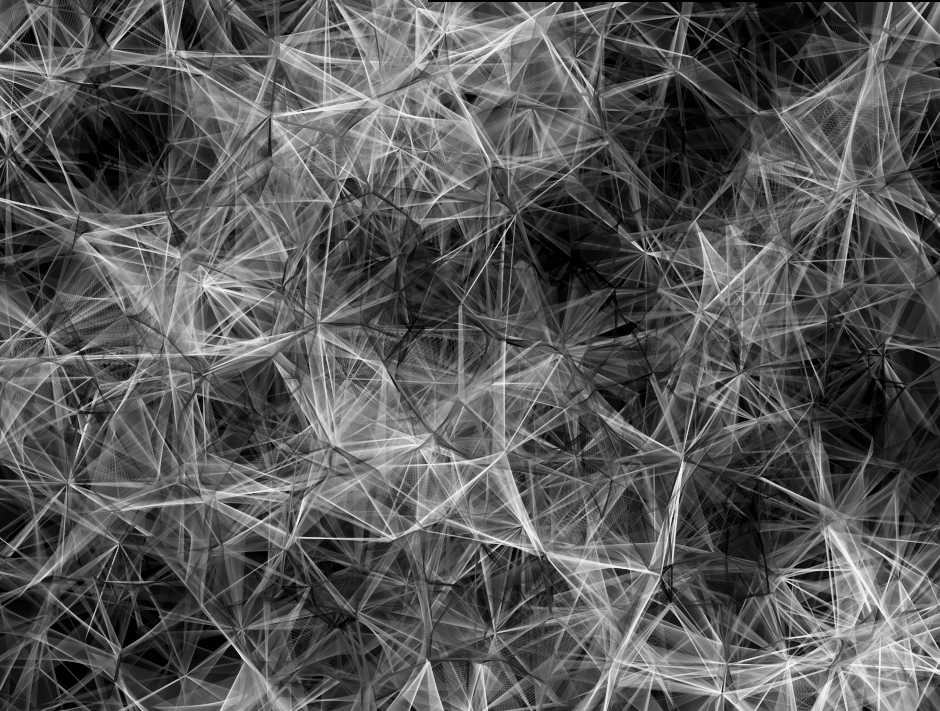
\includegraphics[width=1\paperwidth]{./images/portada.png}}
	\begin{frame}[plain]
		\titlepage
	\end{frame}
}

%\begin{frame}{Introducción}
%\begin{block}{Planteamiento}
%¿Qué vamos a ver?
%\begin{enumerate}
%    \item Transformada de Fourier Discreta (DFT).
%    \begin{enumerate}
%    \item Definición, propiedades y expresión matricial
%    \item Teorema de inversión
%    \item Convolución
%    \item Bidimensional
%    \end{enumerate}
%    \item Transformadas de Fourier Rápidas
%    \item Transformada de Fourier Cuántica
%\end{enumerate}
%\end{block}
%\end{frame}

\section[DFT]{Transformada de Fourier Discreta}
\subsection{Definiciones}

\begin{frame}{}
\begin{block}{Transformada de Fourier (Continua)}
Sea $f \in L_1(\R)$. Recordemos que la transformada de Fourier de $f$ viene dada por
\[
\widehat{f} (\omega )=\int _{-\infty }^\infty e^{-i\omega t}f(t) dt
\]
\end{block}
\begin{block}{Aproximación}
\[
\widehat{f} (\omega ) \approx \int _{a}^b e^{-i\omega t}f(t) dt
\]
\onslide<2->
\[
\widehat{f} (\omega ) \approx \sum _{k=0}^{N-1}f(t_k)e^{-i\omega t_k} (t_{k+1} - t_{k})
\]
con $\{a=t_0<t_1<...<t_{N-1}=b\}$, una partición del intervalo $[a,b]$% y de cardinal $N$
\end{block}
\end{frame}

%\begin{frame}
%\begin{block}{Aproximación}
%\[
%\widehat{f} (\omega ) \approx \int _{a}^b e^{-i\omega t}f(t) dt
%\]
%\onslide<2->
%\[
%\widehat{f} (\omega ) \approx \sum _{k=0}^{N-1}f(t_k)e^{-i\omega t_k} (t_{k+1} - t_{k})
%\]
%con $\{a=t_0<t_1<...<t_{N-1}=b\}$, una partición del intervalo $[a,b]$ y de cardinal $N$
%\end{block}
%\end{frame}

\begin{frame}

%Esta la comento rápidamente para que vean la última aproximación previa a la definición
\begin{block}{No nos perdamos en los detalles}
Para $\Delta t =(b-a)/ N$ tenemos que $t_k=a+k\Delta t$, $k \in \{0,1, \ldots, N-1\}$. Notando $\phi$ a la aproximación de $\widehat{f}$
 \[
 \phi(\omega)=\sum_{k=0}^{N-1} f(t_k)e^{-i\omega t_k }\Delta t=e^{i\omega a}\sum_{k=0}^{N-1} f(t_k)e^{-i\omega k (b-a)/N  }\Delta t.
 \]
 Finalmente, si  $\omega_n=2\pi n / (b-a)$
 \[
 \phi(\omega_n)=e^{i\omega_n a}\sum_{k=0}^{N-1}f(t_k)e^{-i2\pi nk/N}\Delta t,
 \]
\end{block}
\end{frame}

\begin{frame}
\begin{block}{Definición}
Dada $f:\R \longrightarrow \C$ una función se define la \emph{Transformada de Fourier Discreta de $f$} como la aplicación $Df:\Z \longrightarrow \C$ donde, 
 \[
 Df(n) = \sum_{k=0}^{N-1}f(t_k)e^{-i2\pi nk/N},
 \]
\onslide<2->
Notando $\zeta_N=e^{2\pi i/N}$, se tiene
 \[
Df(n) = \sum_{k=0}^{N-1}f(t_k)\zeta_N^{-nk}.
 \]
\end{block}
\begin{block}{Nota}
Nosotros trabajaremos con la Transformada de Fourier Discreta sin normalizar salvo en el caso de la Transformada de Fourier Cuántica. Cuando no haya riesgo de confusión escribiremos $\zeta$ en lugar de $\zeta_N$.
\end{block}
\end{frame}

\begin{frame}
\begin{block}{Discretización}
Supondremos que $f$ está definida en el conjunto $\{ 0,1,\dots ,N-1 \}$
\[
    \begin{array}{rccl}
        f : & \Z _N & \longrightarrow & \C \\
        & k+N\Z & \longmapsto & f(k)
    \end{array}
\]
\onslide<2->
La Transformada de Fourier Discreta (DFT) de $f : \Z _N \to \C $ es la aplicación $D_N f : \Z_N \to \C$ dada por
    \[
        D_N f(n) = \sum_{k=0}^{N-1}f(k)e^{-2\pi ink/N}
    \]
Cuando no haya riesgo de confusión escribiremos $D f$ en lugar de $D_N f$.
\end{block}
\end{frame}
\subsection{Expresión Matricial}
\begin{frame}{Forma matricial}
\begin{block}{Vectores}
\[
Df(n)=\sum_{k=0}^{N-1}f(t_k) \zeta^{-nk}, \hbox{ con }  \zeta=e^{2\pi i/N}
\]
Podemos ver la función $f$ y su trasformada $Df$ como vectores
\[
Df=\begin{pmatrix}
Df(0)\\ \vdots \\Df(N-1)\\
\end{pmatrix}
, \quad
f=\begin{pmatrix}
f(0)\\ \vdots \\f(N-1)\\
\end{pmatrix}
\]
\end{block}
\end{frame}

\begin{frame}
\begin{block}{Matriz}
Notando que $\zeta^N = 1$ y que $\overline{\zeta} = \zeta ^{-1}$, definimos la matriz
\[
M_{N}=\begin{pmatrix}
1&1&1&\dots&1 \\
1&\overline{ \zeta}&\overline{ \zeta}^{2}&\cdots&\overline{ \zeta}^{N-1}\\
1&\overline{ \zeta}^{2}&\overline{ \zeta}^{4}&\cdots&\overline{ \zeta}^{N-2}\\
\vdots&\vdots&\vdots&\ddots&\vdots\\
1&\overline{ \zeta}^{N-1}&\overline{ \zeta}^{N-2}&\cdots&\overline{ \zeta}\\
\end{pmatrix}
\]
Observamos que esta matriz es simétrica.
A partir de la definición de DFT es fácil ver que $Df = M_Nf$.
\end{block}
\end{frame}

\begin{frame}
\begin{block}{Vandermonde}
Nótese que $M_N$ es una matriz de Vardenmonde.
\[
V(x_{0},\dots,x_{n})=\begin{pmatrix}
1&x_{0}&x_{0}^{2}&\dots&x_{0}^{n} \\
1&x_{1}&x_{1}^{2}&\dots&x_{1}^{n} \\
\vdots&\vdots&\vdots&\ddots&\vdots\\
1&x_{n}&x_{n}^{2}&\dots&x_{n}^{n} \\
\end{pmatrix}
\]
\end{block}
\onslide<2->
\begin{block}{Determinante}
En nuestro caso, para la matriz $M_N$, $x_k=\overline{\zeta}^k \quad \forall k \in \{0, \dots, N-1\}$. 
Recordemos que el determinante de una matriz de Vandermonde es $\prod_{i>j}(x_i-x_j)$.
\[
\det(M_N)=\prod_{i>j}(\zeta^{-i}-\zeta^{-j}),
\]
que es distinto de $0$ ya que $\zeta^{-i} \ne \zeta^{-j}$ para todo $i \ne j$.
\end{block}
\end{frame}

\begin{frame}{Teorema}
    \begin{theorem}[Teorema de Inversión]
    Sea $f:\Z_N \rightarrow \C$, con Transformada de Fourier Discreta dada por
    \[
        Df(n) = \sum_{k=0}^{N-1}f(k)e^{-2\pi ink /N} = \sum_{k=0}^{N-1} f(k)  \zeta ^{-kn},
    \]
    Entonces, se tiene que
    \[
        f(n) = \frac{1}{N} \sum_{k=0}^{N-1} Df(k)e^{2\pi ink / N} = \frac{1}{N} \sum_{k=0}^{N-1} Df(k) \zeta ^{kn}.
    \]
\end{theorem}
\end{frame}

\begin{frame}
\begin{block}{Definición}
Definimos para cada $j \in \{0,\dots,N-1\}$ la función $\zeta_j : \Z_N \to \C$ dada por $\zeta_j(m)= \zeta^{-jm}$ para todo $m \in \{0,1,\ldots,N-1\}$.
Al igual que con $f$ y $Df$ podemos ver esta familia de funciones como los vectores
\[ \zeta_j = \left( 1, \zeta^{-j}, \zeta^{-2j}, \dots , \zeta^{-(N-1)j} \right).\]
\end{block}
\end{frame}

%Este lema diré que es álgebra y que todo el mundo lo conoce
\begin{frame}
\begin{lemma}{}
Sea $N \in \N$ con $N\geq 2$. Consideremos las raíces $N$-ésimas de la unidad dadas por $\zeta^m = e^{2\pi im / N}$ para $m \in \left\{ 1,2, 		\dots , N-1\right\} $. Entonces
\[
\sum_{k=0}^{N-1}\zeta ^k = 0.
\]
\end{lemma}
\onslide<2->
\begin{lemma}{}
El conjunto $\left\{ \zeta_j / \sqrt{N} : j=0,\dots ,N-1\right\} $ es una base ortonormal de $L_1(\Z_N).$
\end{lemma}
\end{frame}

%La demostración del lema son dos diapositivas. Las paso de puntillas para que se vea que son cuentas y es básicamente usar el primer lema
\begin{frame}
\begin{block}{Demostración del lema}
  Puesto que $L_1(\Z_N)$ es un espacio de dimensión $N$ basta probar que para cualquier pareja $k,j \in \{0,1,\ldots,N-1\}$ se verifica
  \[
  \langle \frac{1}{\sqrt{N}} \zeta_j,\frac{1}{\sqrt{N}} \zeta_k\rangle=\delta_{kj}.
  \]
  En efecto, nótese que
  \[
  \langle \frac{1}{\sqrt{N}} \zeta_j,\frac{1}{\sqrt{N}} \zeta_k\rangle=\frac{1}{N}\langle \zeta_j, \zeta_k\rangle=\frac{1}{N}\sum_{n=0}^{N-1} \zeta_j(n)\overline{ \zeta_k(n)}=\frac{1}{N}\sum_{n=0}^{N-1} \zeta^{(k-j)n}.
  \]
\end{block}
\end{frame}

\begin{frame}
\begin{block}{Demostración del lema}
  Si $j=k$ tenemos que,
  \[\frac{1}{N}\sum_{n=0}^{N-1} \zeta^{(k-j)n}=\frac{1}{N}\sum_{n=0}^{N-1} \zeta^{0}=1.\]
  Si $j\neq k$ entonces por el Lema anterior para $m=k-j$ obtenemos
  \[\frac{1}{N}\sum_{n=0}^{N-1}\zeta^{(k-j)n}=\frac{1}{N}\sum_{n=0}^{N-1}\left(\zeta^m\right)^n=0. \]
\end{block}
\end{frame}

\begin{frame}
\begin{block}{Demostración del teorema}
Se tiene que las filas de la matriz $M_N$ son
\[
    M_{N} = \begin{pmatrix}
     \zeta_0 \\
     \zeta_1 \\
    \vdots \\
     \zeta_{N-1} \\
    \end{pmatrix}.
\]
Por tanto, la matriz $M_N / \sqrt{N}$ tiene por filas a los elementos de la base ortonormal del lema. Así, tenemos que
\begin{align*}
    \frac{M_N}{\sqrt{N}} \frac{M_N^{\ast}}{\sqrt{N}} &= {\bf I} \\
    M_N M_N^{\ast} &= N{\bf I}
\end{align*}
Donde $M_N^{\ast}$ es la matriz adjunta de $M_N$.
\end{block}
\end{frame}

%\begin{frame}
%\begin{block}{Demostración del teorema}
%\[
%    M_N M_N^* = \begin{pmatrix}
%    N & 0 & 0 & \dots & 0 \\
%    0 & N & 0 & \cdots & 0 \\
%    0 & 0 & N & \cdots & 0 \\
%    \vdots & \vdots & \vdots & \ddots & \vdots \\
%    0 & 0 & 0 & \cdots & N \\
%    \end{pmatrix} = N{\bf I}
%\]
%\end{block}
%\end{frame}

\begin{frame}
\begin{block}{Demostración del teorema}
Como la matriz inversa de $M_N$ existe, pues $M_N$ tiene determinante no nulo, nos queda
\[
    \frac{1}{N}M_N^{\ast} = M_N^{-1}.
\]
\onslide<2->
Finalmente, como $Df = M_N f$, se obtiene:
\begin{align*}
	f &= M_N^{-1}Df = \frac{1}{N}M_N^{\ast}Df \\
	f(n) &= \frac{1}{N} \sum_{k=0}^{N-1} Df(k) \zeta ^{kn}. 
\end{align*}
\end{block}
\end{frame}

%David elige si comentar las propiedades o no

%\begin{frame}
%\begin{block}{Propiedades}
%Fijemos $j \in \Z$ y sea $f:\Z_N \longrightarrow \C$. Se verifican las siguientes afirmaciones:
%\begin{enumerate}
%    \item La DFT de $f(n-j)$ es $Df(n) \zeta^{-jn}$.
%    \item La DFT de $f(n) \zeta^{jn}$ es $Df(n-j)$.
%    \item La DFT de $f(n)\cos(2\pi jn/N)$ es $(Df(n-j)+Df(n+j)) / 2$.
%\end{enumerate}
%\end{block}
%\end{frame}

%David elige si comentar las propiedades o no
%Esto no da tiempo
\section{Convolución}
\subsection{Definición}
\begin{frame}{Convolución Continua}
\begin{block}{Definición}
Sean $f,g \in L_1(\R^N)$ se define la convolución de $f$ y $g$ como la función $f \ast g \in L_1(\R^N)$ dada por
\[
(f\ast g)(x)=\int_{\R^N}f(y)g(x-y)dy
\]
para todo $k \in \R^N$.
\end{block}

\end{frame}

\begin{frame}{Convolución Discreta}
\begin{block}{Definición}
Sean $f,g \in L_1(\Z_N)$ se define la convolución de $f$ y $g$ como la función $f \ast g \in L_1(\Z_N)$ dada por
\[
(f\ast g)(k)=\sum_{j=0}^{N-1}f(j)g(k-j)
\]
para todo $k \in \Z_N$.
\end{block}

\end{frame}

\begin{frame}
\begin{block}{Propiedades}
Sean $f,g,h \in L_1(\Z_N)$. Se verifican las siguientes afirmaciones:
\begin{enumerate}[<+-|alert@+>]
    \item $f\ast g=g\ast f$;
    \item $f\ast (g\ast h)=(f\ast g)\ast h$;
    \item $a(f\ast g)=(af)\ast g$ con $a \in \R$;
    \item $f\ast(g+h)=f\ast g+f\ast h$.
\end{enumerate}
\end{block}

\end{frame}

\begin{frame}
\begin{alertblock}{Teorema}
 Para $f,g \in L_1(\Z_N)$ se verifica que $D(f \ast g)(n)=Df(n)Dg(n)$ para todo $n \in \Z_N$.
\end{alertblock}

\end{frame}
\begin{frame}
\begin{proof}%%No voy a demostrarla solo es para que vean que ocupa poco
 Sea $n \in \Z_N$. Tenemos que
\[
    D(f\ast g)(n) = \sum_{k=0}^{N-1}f \ast g(k)e^{-2\pi ikn/N}
    =\sum_{k=0}^{N-1} f \ast g(k)\zeta^{-kn}
\]
\[=\sum_{k=0}^{N-1} \left(\sum_{j=0}^{N-1} f(j)g(k-j)\right)\zeta^{-kn}
    =\sum_{j=0}^{N-1}f(j)\left(\sum_{k=0}^{N-1}g(k-j)\zeta^{-kn}\right)
\]
\[=\sum_{j=0}^{N-1} f(j)\zeta^{jn}\left(\sum_{k=0}^{N-1}g(k-j)\zeta^{-(k-j)n}\right)
    =Df(n)Dg(n). \qedhere
 \]
\end{proof}
	\begin{center}
		\begin{Large}
		\onslide<2>{¡Sin usar ningún teorema de tipo Fubini!}
		\end{Large}
	\end{center}
\end{frame}

\begin{frame}{Una sorpresa}

No existe la unidad para la convolución cuando trabajábamos en $L_1(\R^n)$. En nuestro caso, $L_1(\Z_N)$ si que tenemos una función que actúa como unidad:
\[
e(k)=(1,0,\dots,0),
\]
con la que tenemos simplemente aplicando la definición que $f \ast e=f \quad \forall f \in L_1(\Z_N)$.

\only<2>{
\[
(f\ast g)(k)=\sum_{j=0}^{N-1}f(j)g(k-j)
\]
}
\only<3>{
\[
(f\ast e)(k)=\sum_{j=0}^{N-1}f(j)e(k-j)
\]
}

\end{frame}

\subsection{Ejemplo}

\begin{frame}{Un ejemplo}
\only<1>{
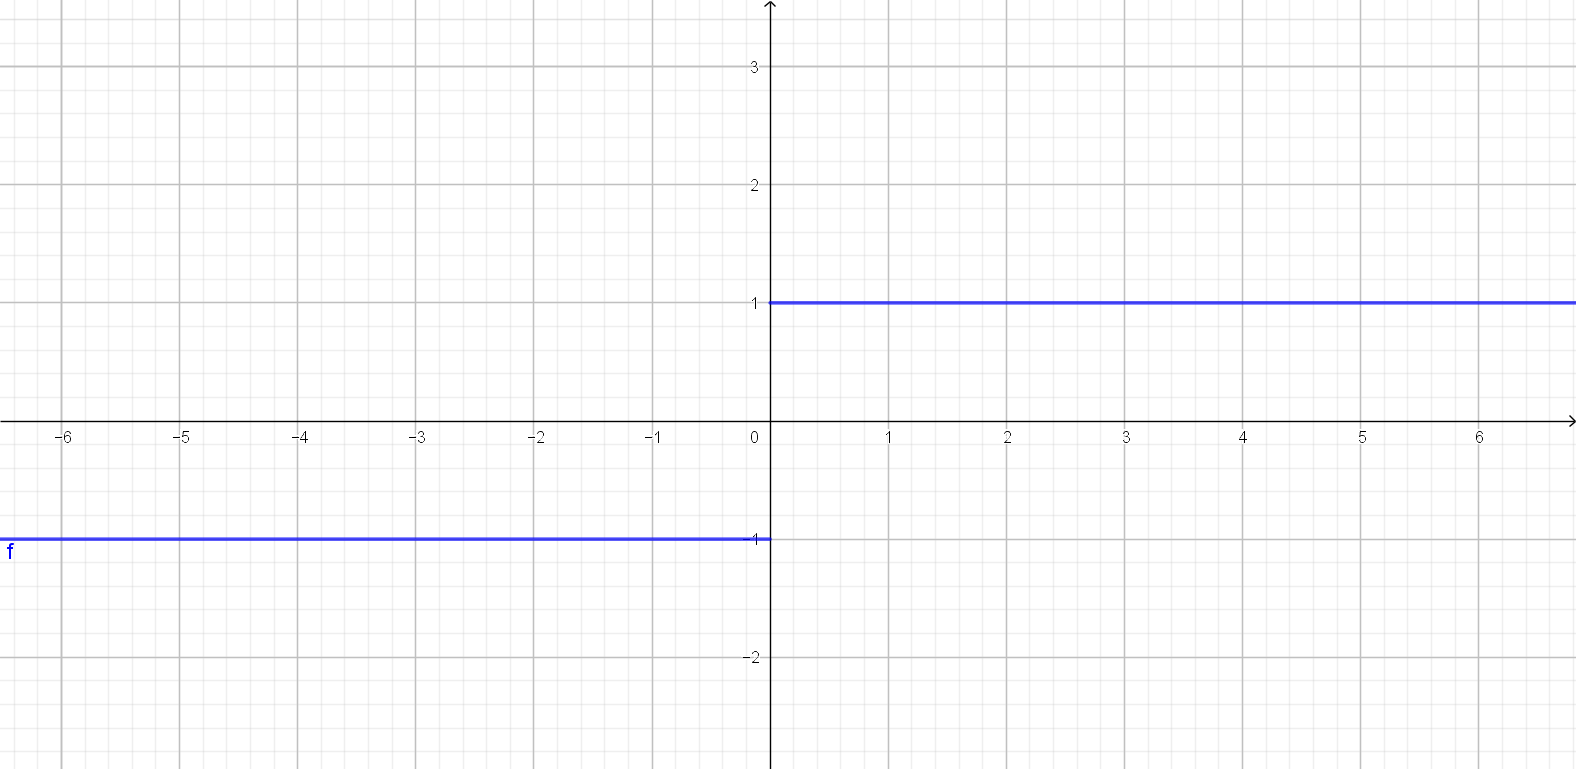
\includegraphics[scale=0.8]{./images/4.png}
}
\only<2>{
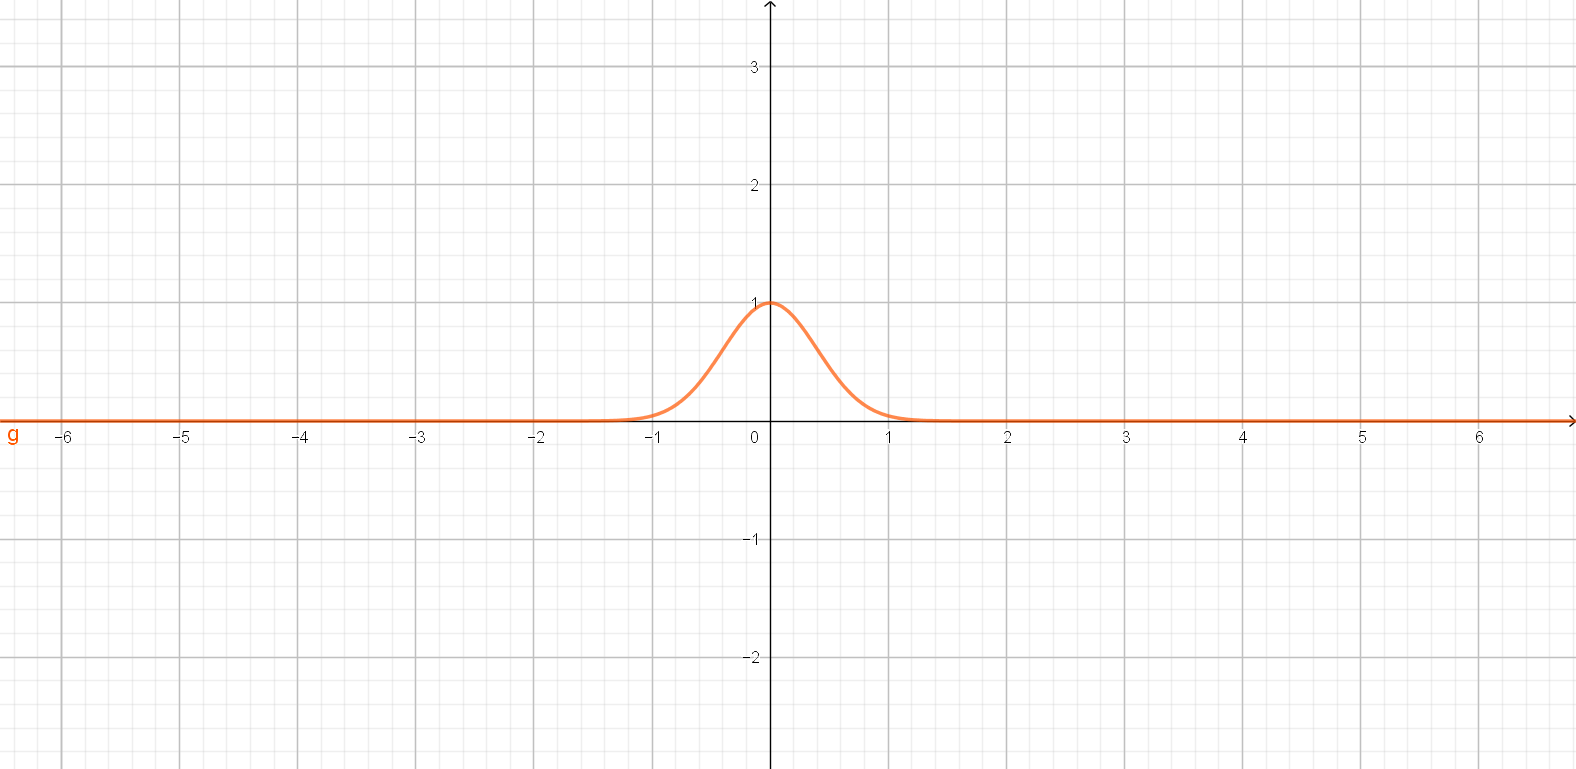
\includegraphics[scale=0.8]{./images/3.png}
}
\only<3>{
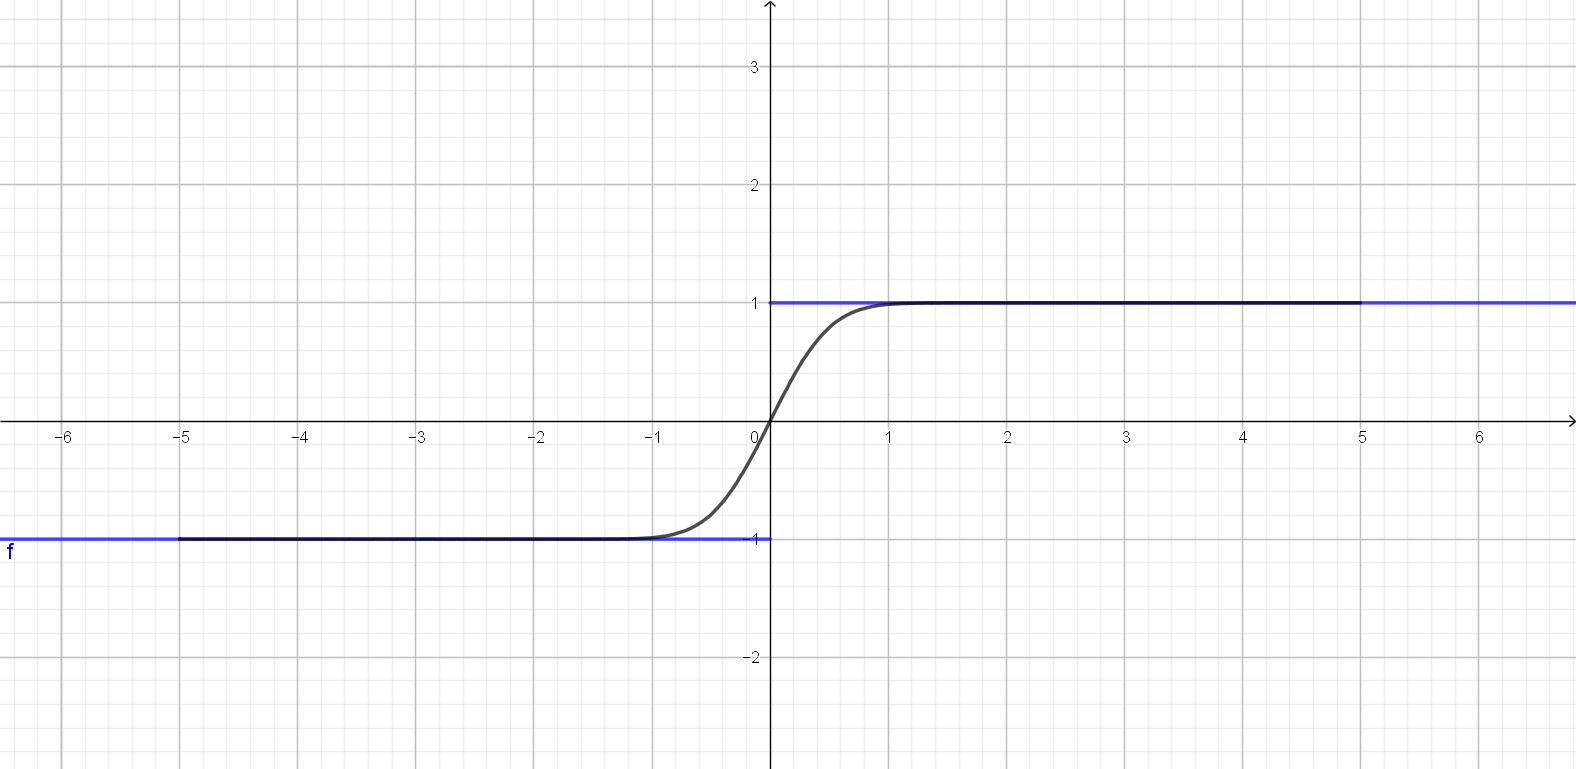
\includegraphics[scale=0.8]{./images/1.png}
}
\only<4>{
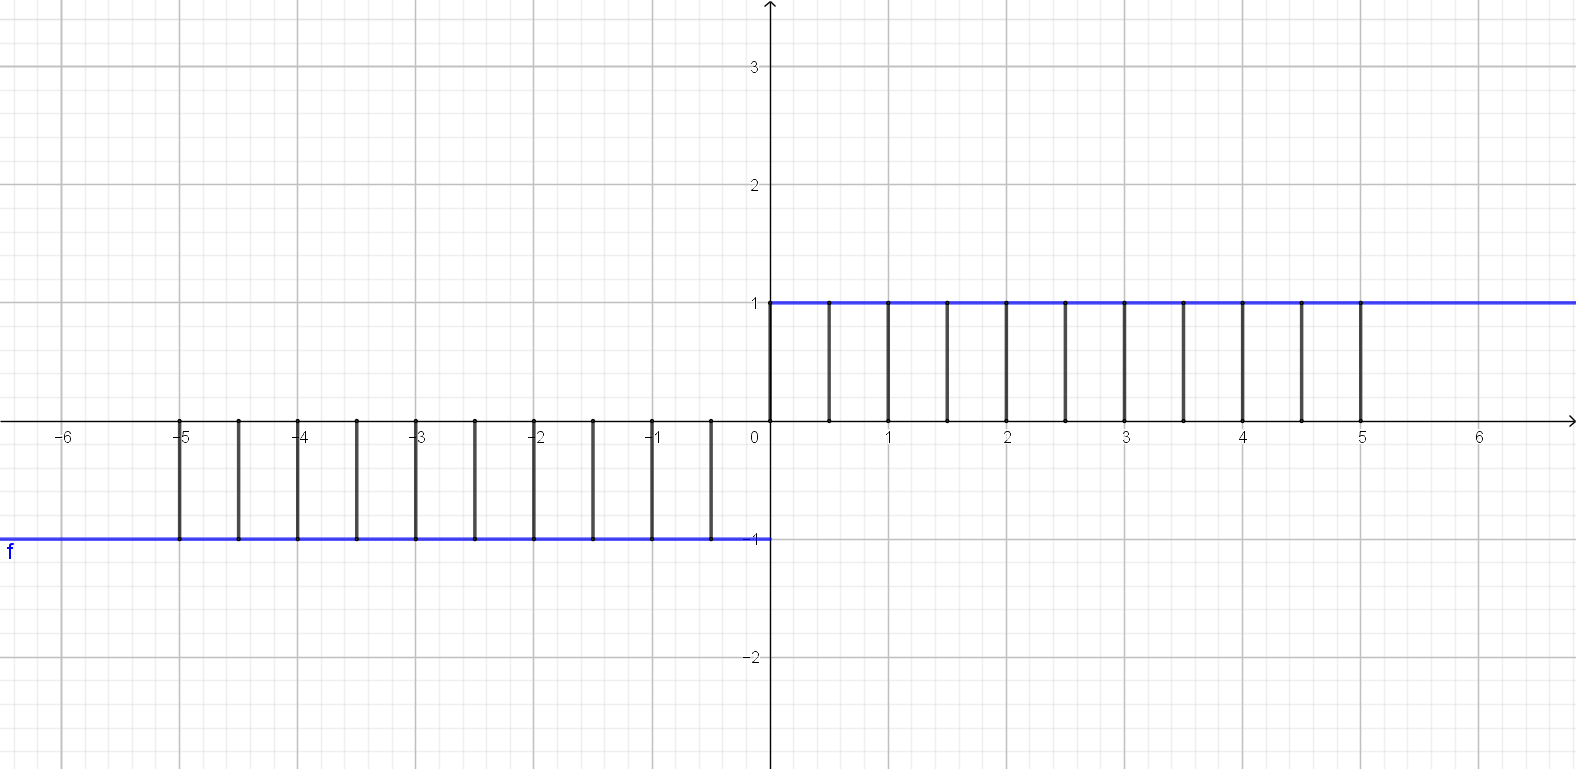
\includegraphics[scale=0.8]{./images/2.png}
}
\only<5>{
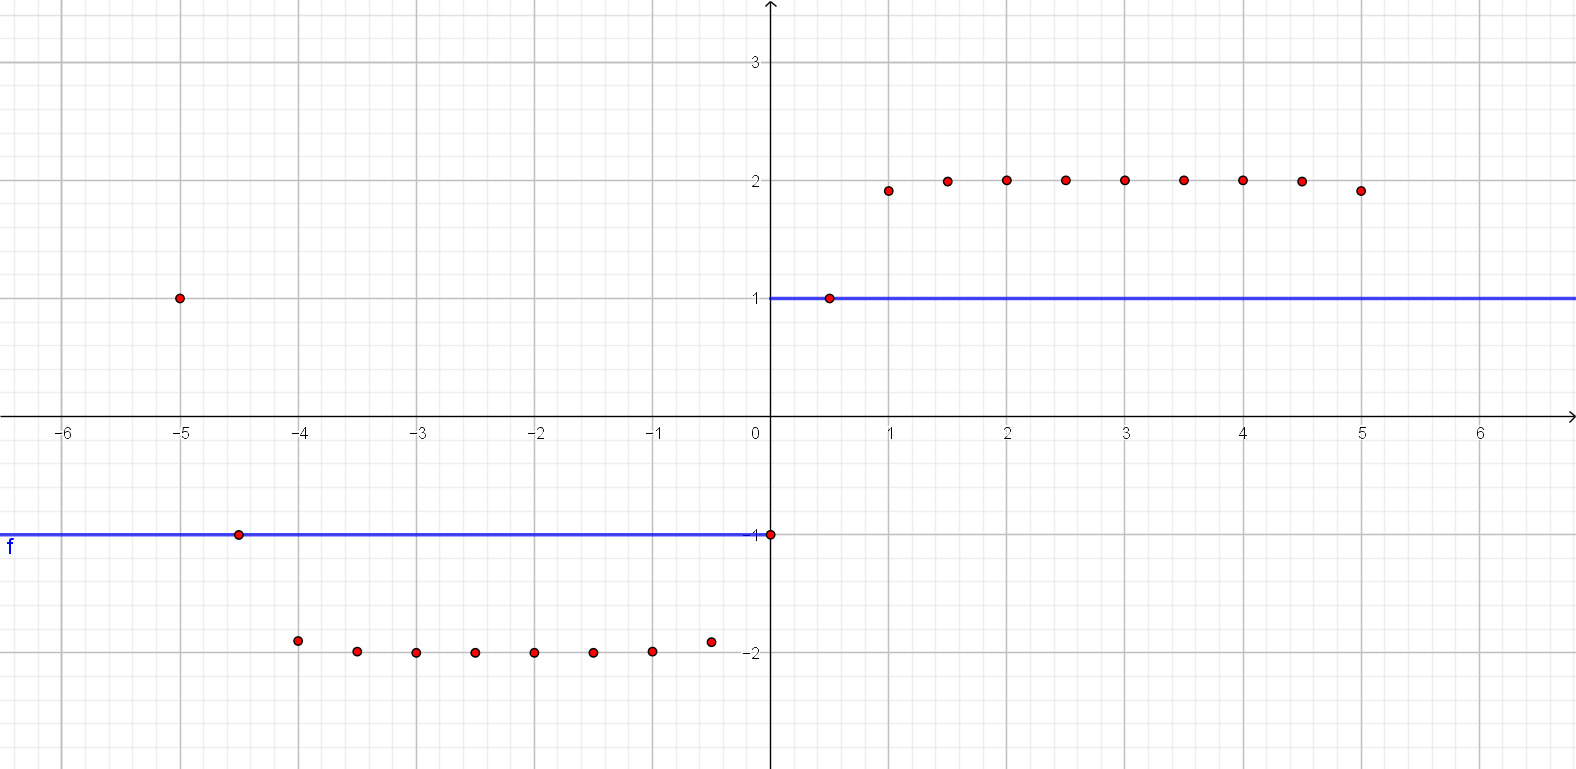
\includegraphics[scale=0.8]{./images/Ult.png}
}
\end{frame}

\section{DFT Bidimensional}

\subsection{Transformada de Fourier Discreta Bidimensional}

\begin{frame}{Transformada Bidimensional}
\only<1>{
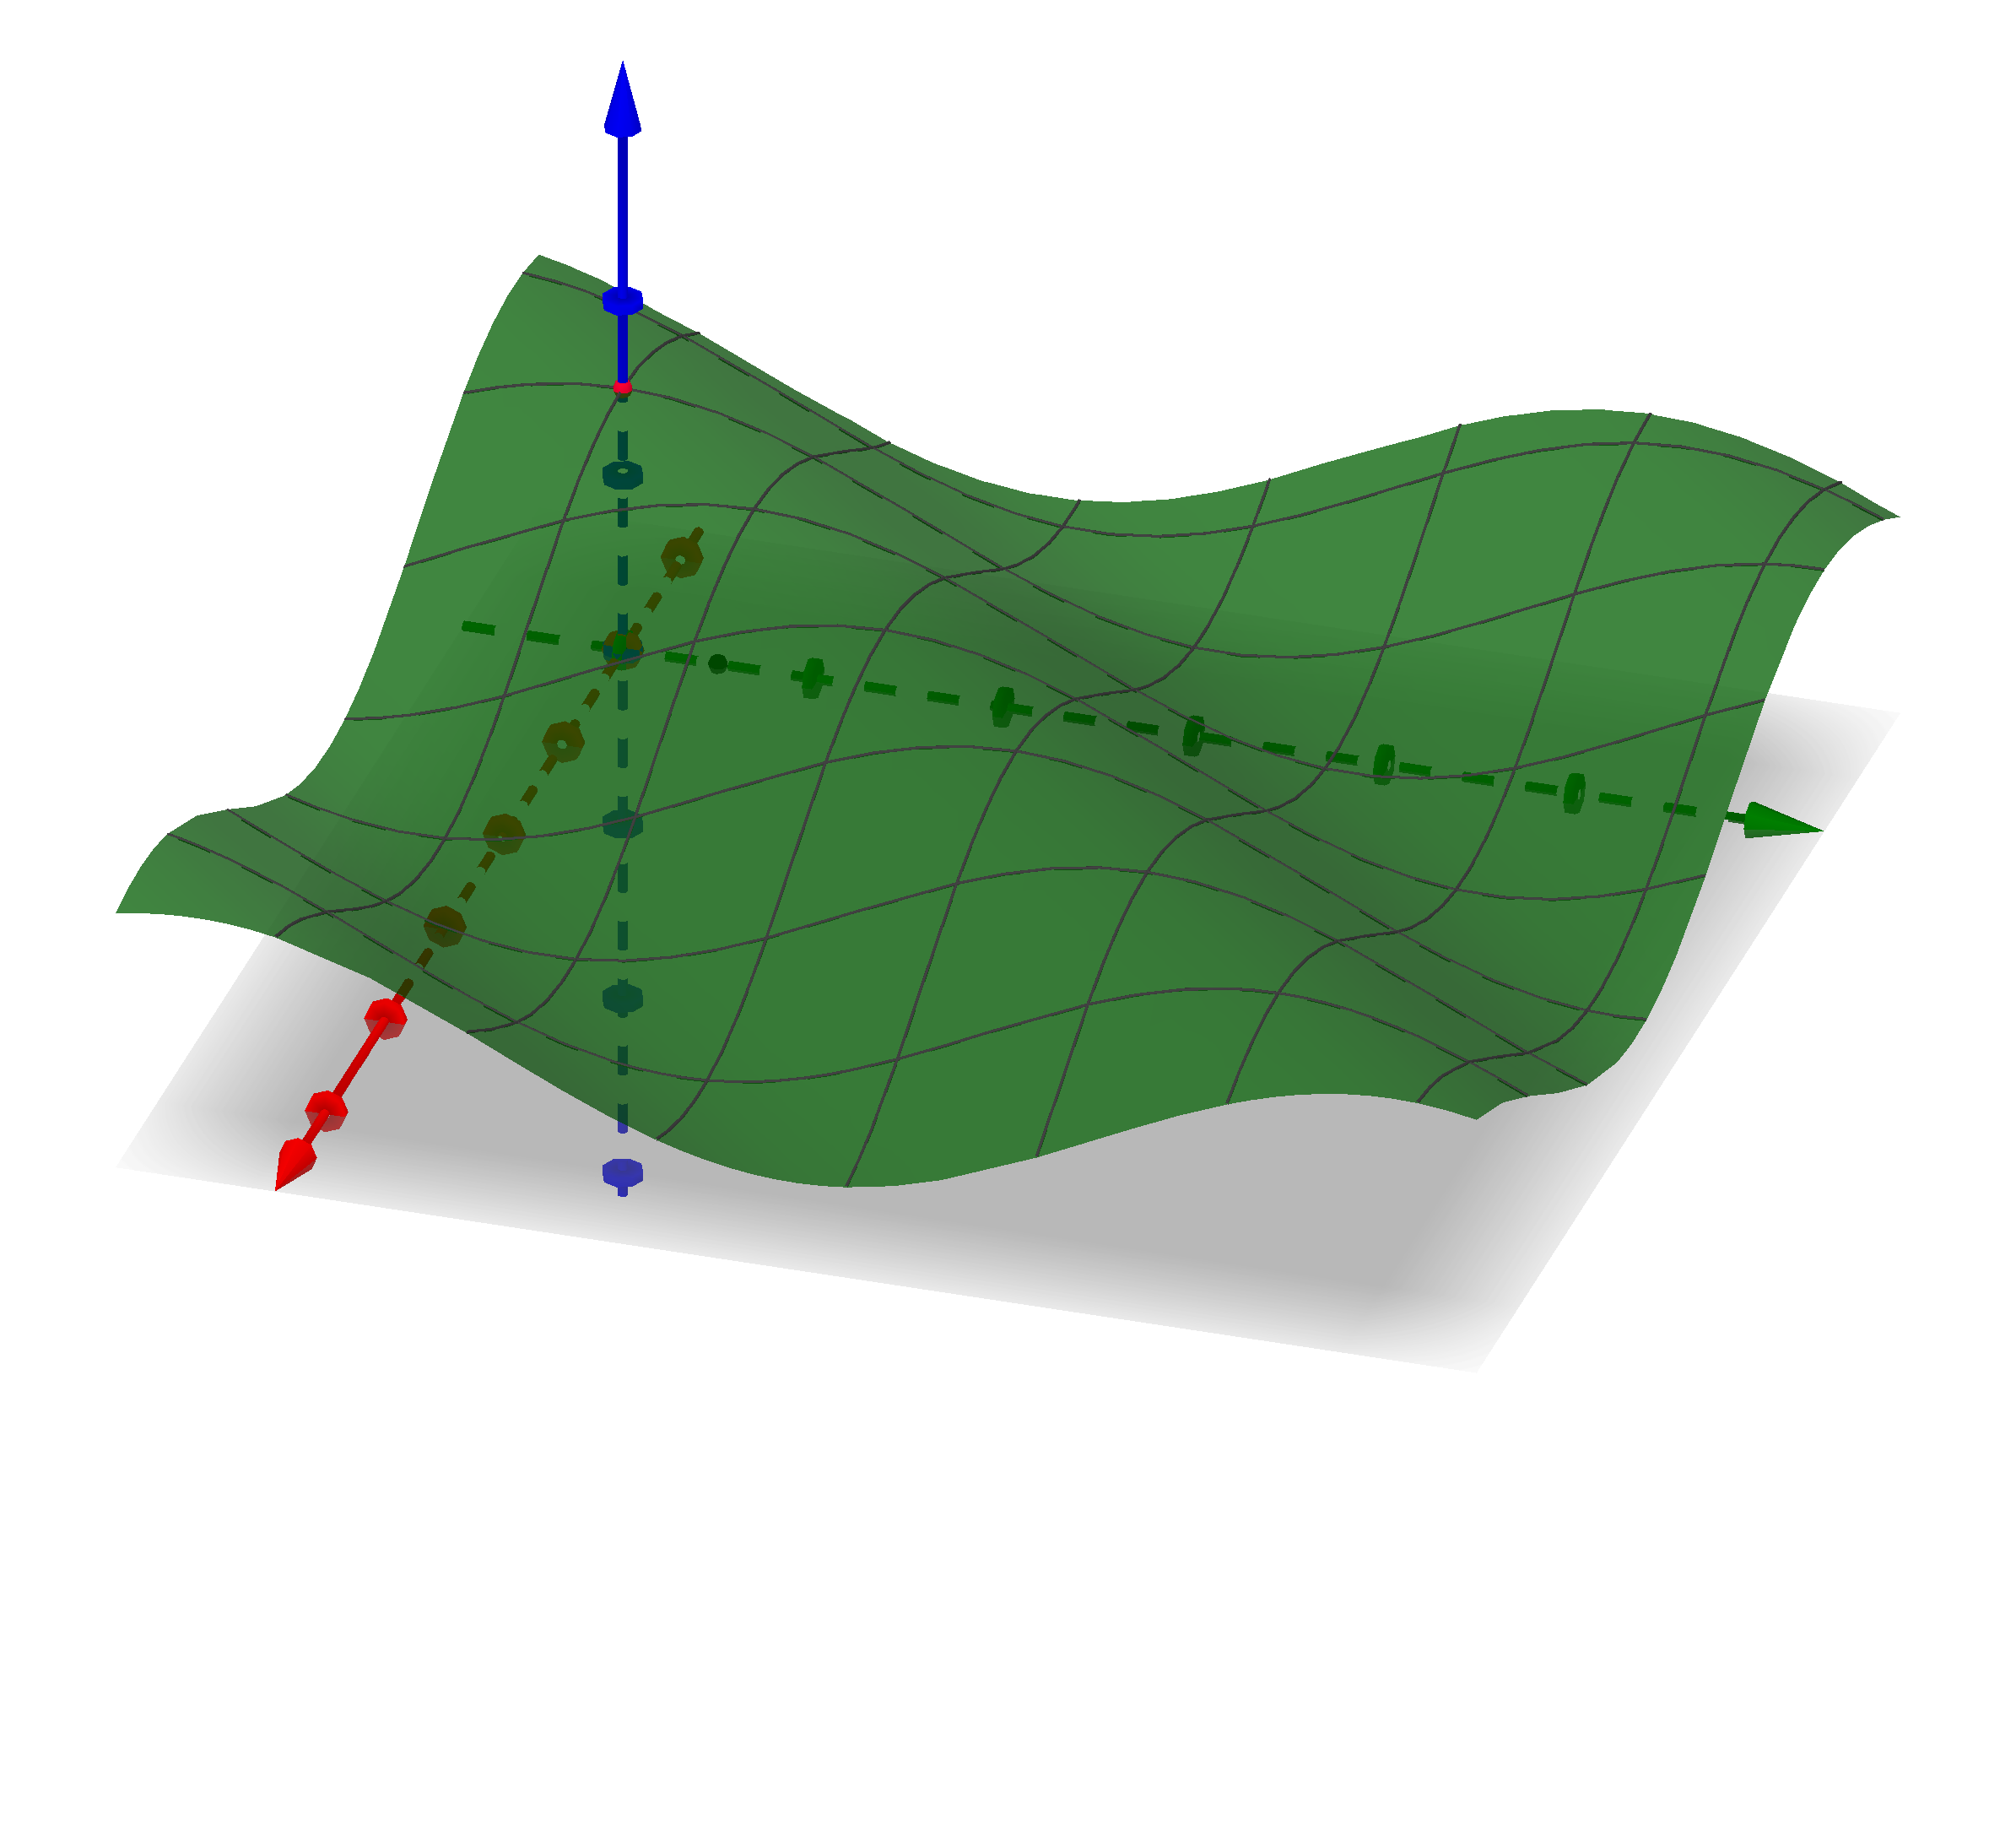
\includegraphics[scale=0.5]{./images/s1.png}
}
\only<2>{
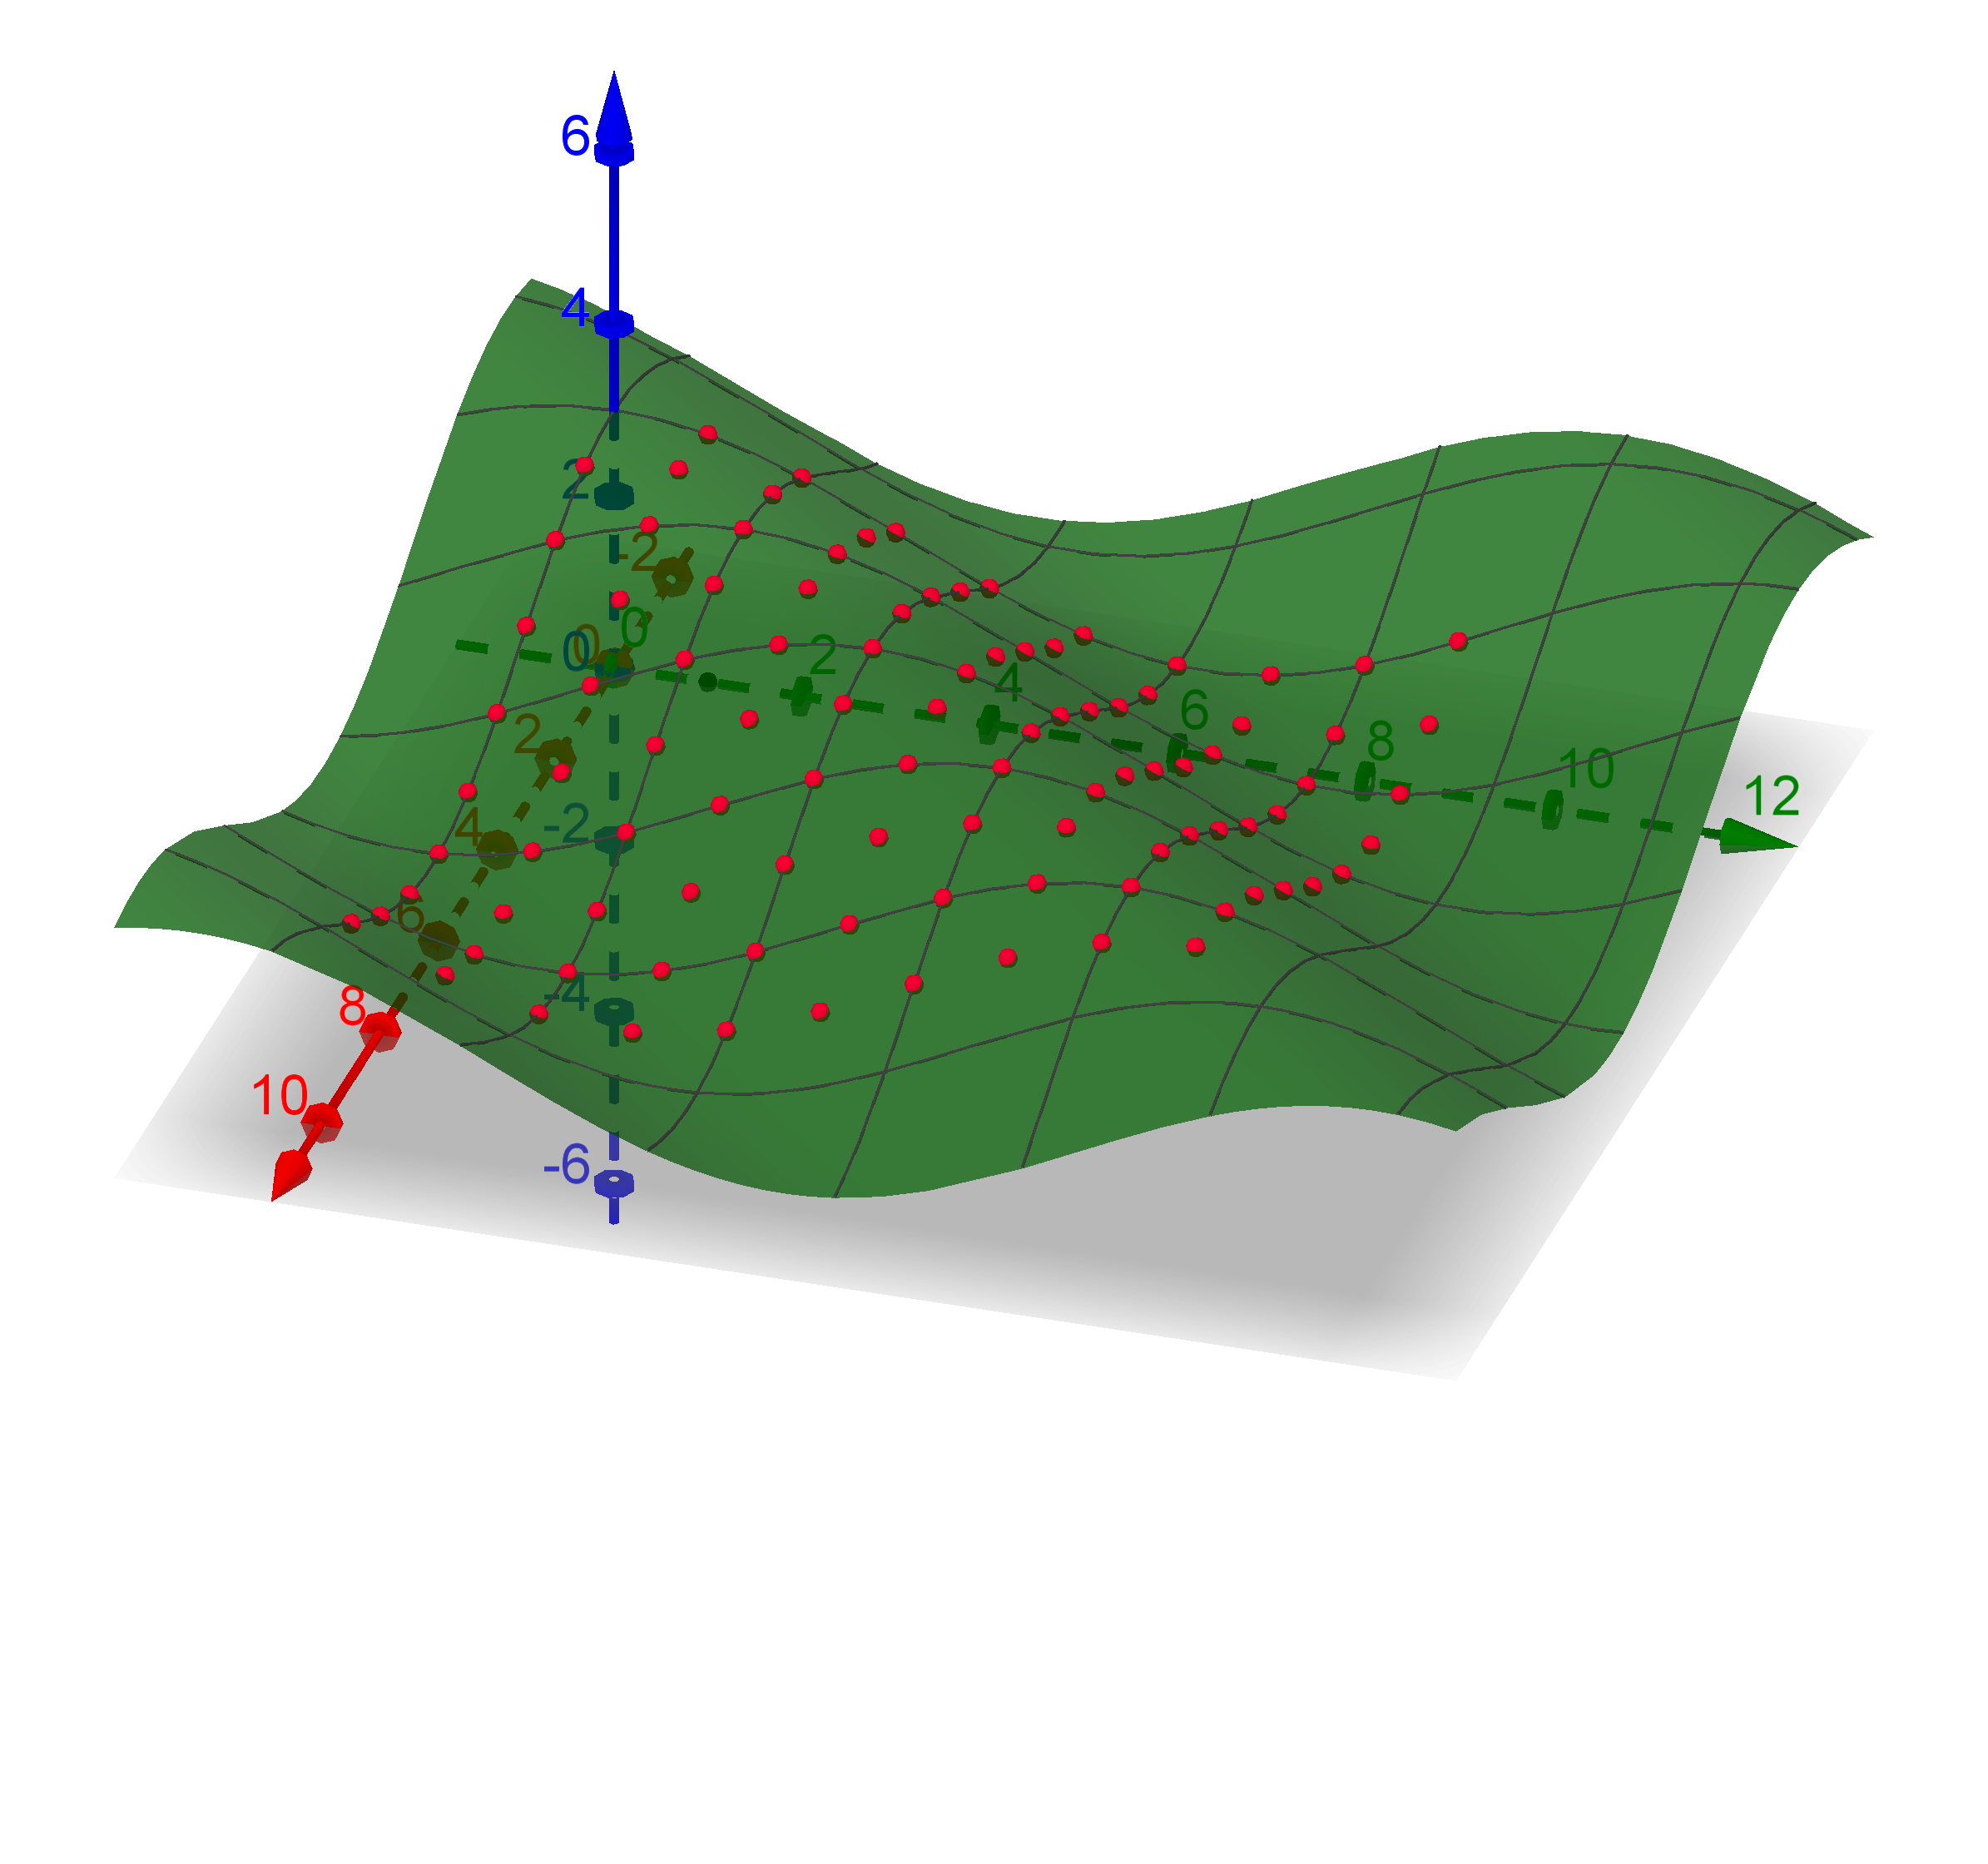
\includegraphics[scale=0.5]{./images/s2.png}
}
\only<3>{
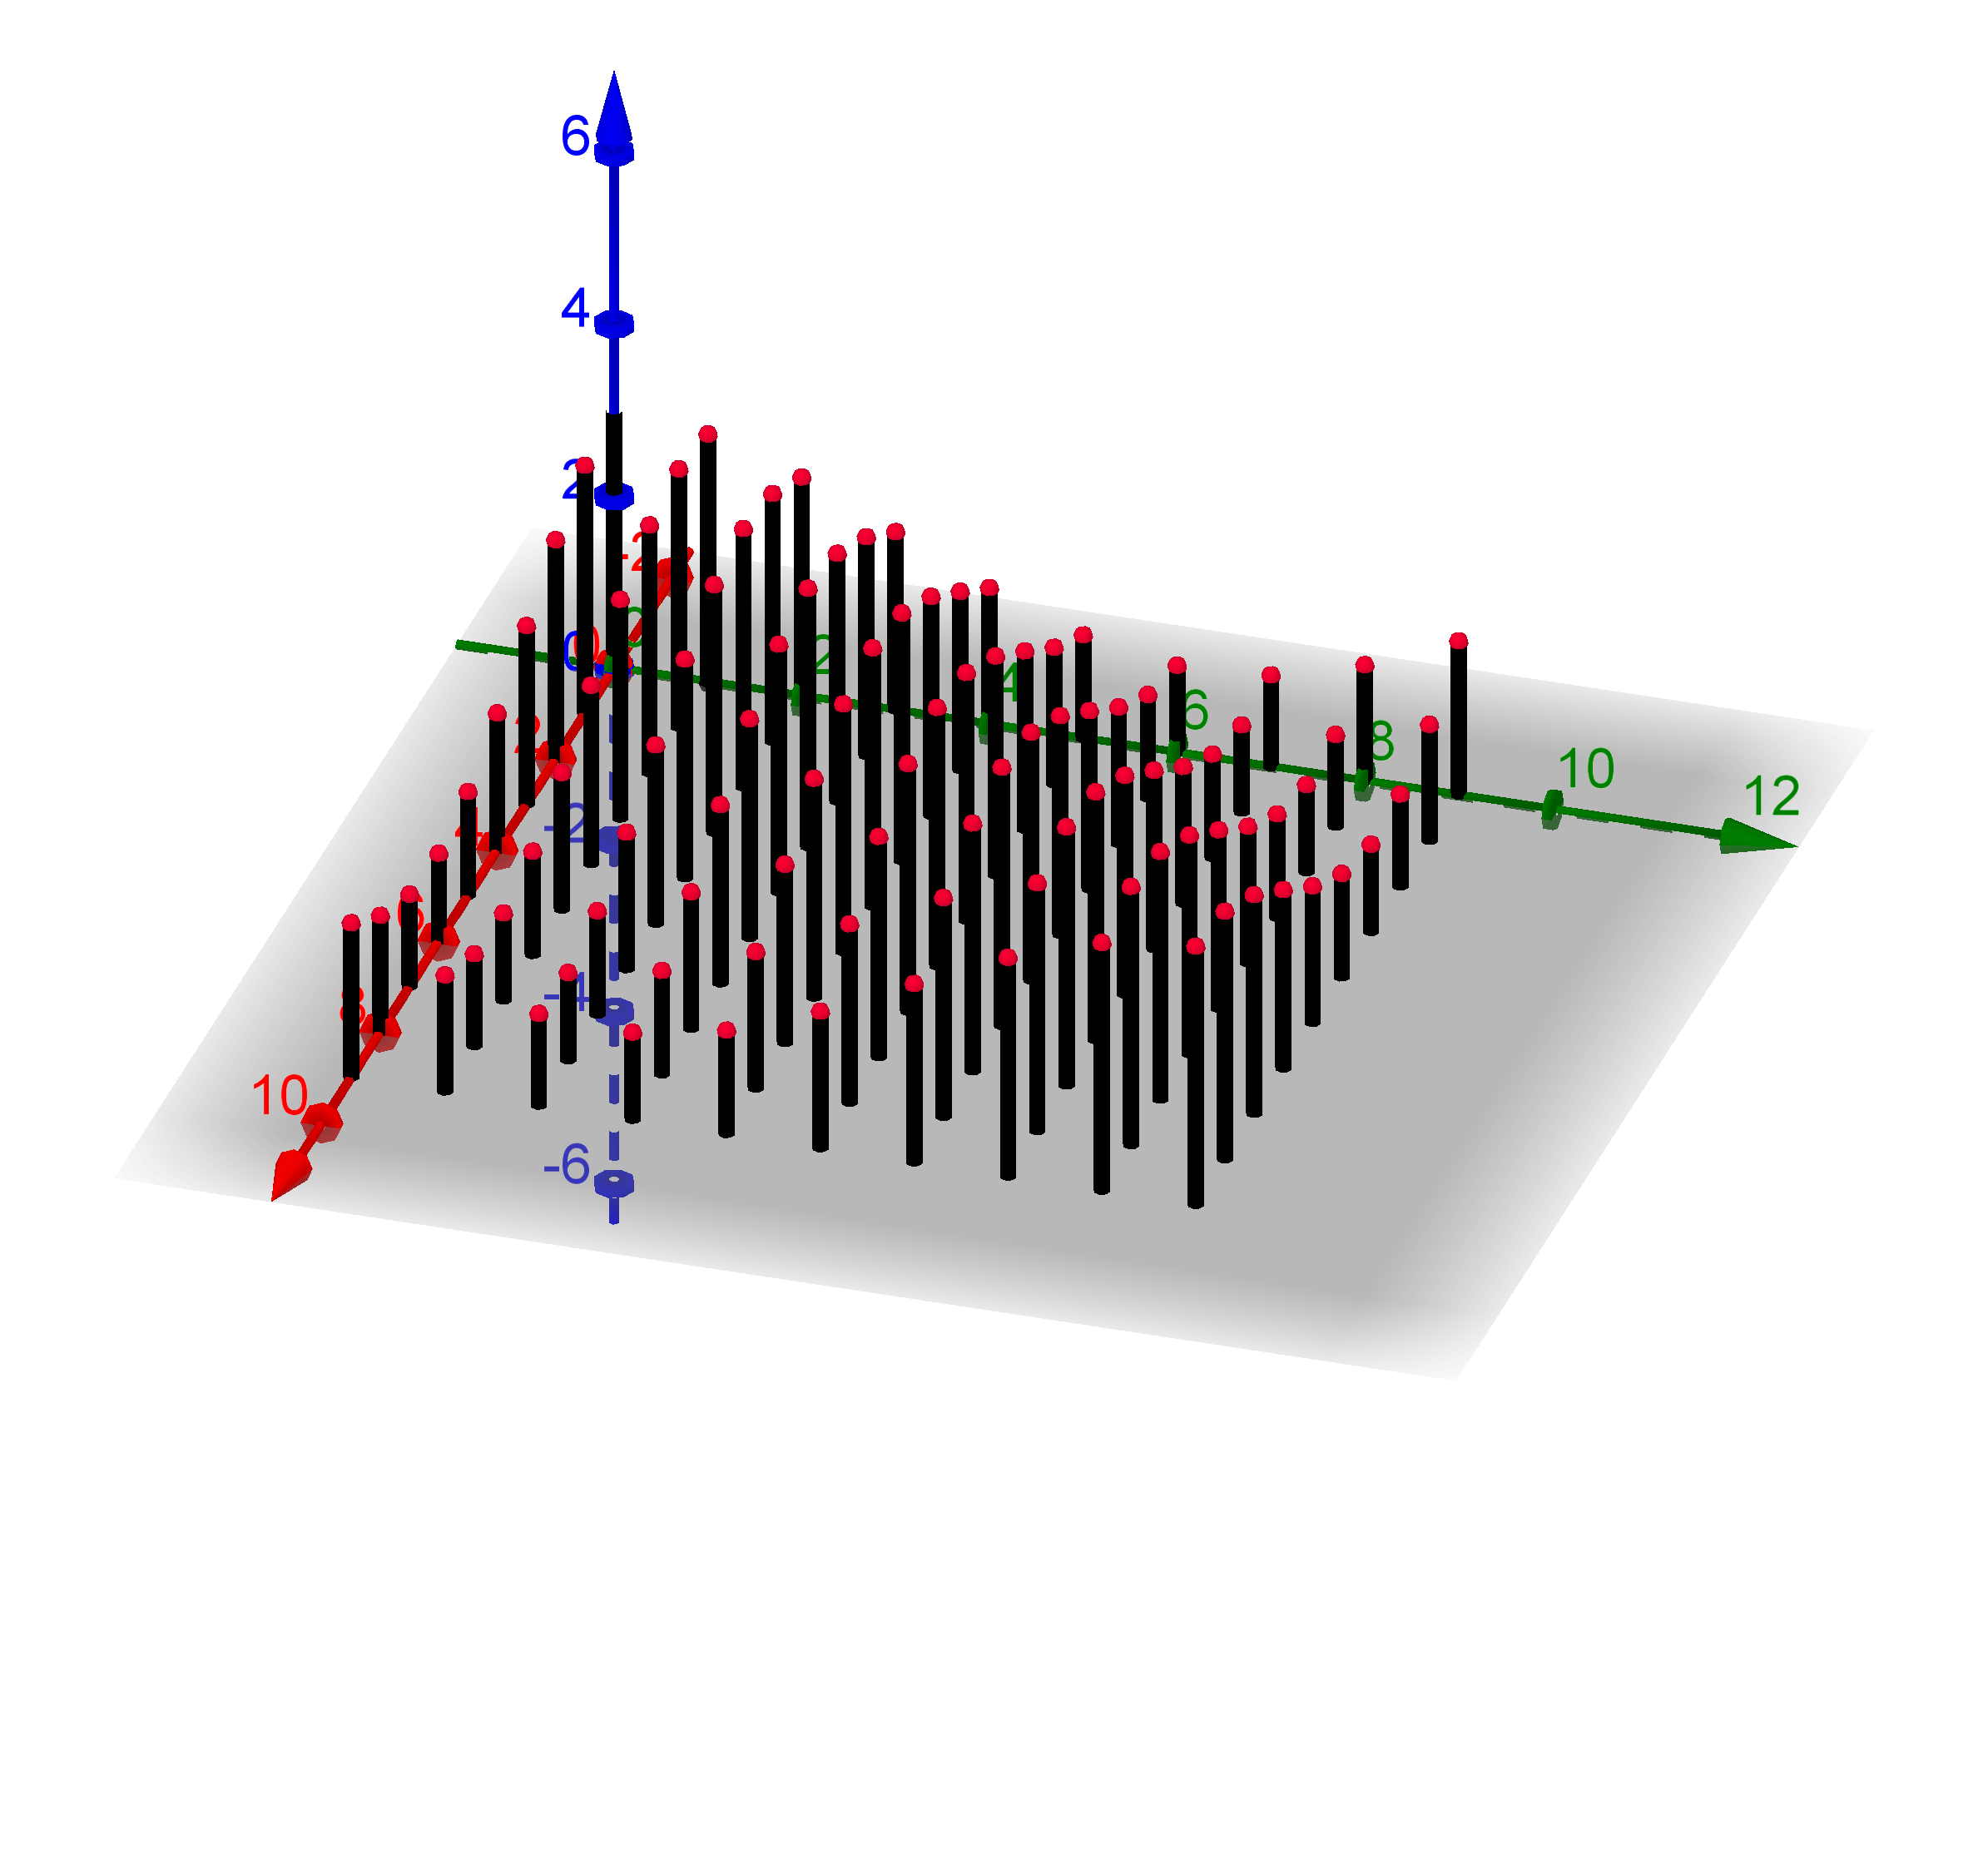
\includegraphics[scale=0.5]{./images/s3.png}
}
\end{frame}

\begin{frame}
\begin{block}{Notación matricial}
Vemos a las funciones como matrices:
\[
    (f) = \begin{pmatrix}
    f(0,0) & f(0,1) & \dots & f(0,N-1) \\
    f(1,0) & f(1,1) & \dots & f(1,N-1) \\
    \vdots & \vdots & \ddots & \vdots \\
    f(N-1,0) & f(N-1,1) & \dots & f(N-1,N-1) \\
    \end{pmatrix}
\]
\end{block}
\end{frame}

\begin{frame}
\begin{block}{Definición}
     $N_1, N_2 \in \mathbb{N}$, $ \zeta_{N_{1}} = e^{2\pi i / N_1}$ y $ \zeta_{N_{2}} = e^{2\pi i / N_2}$.  
    \[
        Df(n_1, n_2) = \sum_{k_1=0}^{N_1 - 1}\sum_{k_2=0}^{N_2 - 1} f(k_1, k_2) \zeta_{N_{1}}^{-n_1k_1}  \zeta_{N_{2}}^{-n_2k_2} 
    \]
     $n_1 \in \{ 0,1,\dots , N_1 - 1\}$ y $n_2 \in \{ 0,1,\dots , N_2 - 1\}$
\end{block}
\end{frame}

\begin{frame}
\begin{block}{Notación matricial}
\[
    (Df) = \begin{pmatrix}
    Df(0,0) & Df(0,1) & \dots & Df(0,N-1) \\
    Df(1,0) & Df(1,1) & \dots & Df(1,N-1) \\
    \vdots & \vdots & \ddots & \vdots \\
    Df(N-1,0) & Df(N-1,1) & \dots & Df(N-1,N-1) \\
    \end{pmatrix}
\]
\end{block}
\end{frame}

\begin{frame}
Así, las expresiones matriciales para el caso de dos dimensiones $N \times N$ vienen dadas por:
\[
    (Df) = M_N (f) M_N ,
\]
de donde podemos deducir el teorema de inversión.
\begin{alertblock}{Teorema de Inversión}
\[(f) = \frac{1}{N^2} M_N^{\ast} (Df) M_N^{\ast}\]
\end{alertblock}
\begin{proof}
\[\frac{1}{N^2} M_N^{\ast} (Df) M_N^{\ast}=\frac{1}{N^2} M_N^{\ast} M_N (f) M_N  M_N^{\ast}=\frac{N}{N^2}(f)N=f\]
\end{proof}
\end{frame}

% \begin{block} {Identidad de Parceval}
% 	\[\sum^{N-1}_{n_1=0}\sum^{N-1}_{n_2=0}|f(n_1,n_2)|^2=\frac{1}{N%^2}\sum^{N-1}_{k_1=0}\sum^{N-1}_{k_2=0}|Df(k_1,k_2)|^2\]
% 	\end{block}
%\end{frame}
%Recortando tiempo

\begin{frame}
\begin{block}{Definición}
Sean así $f,g \in L_1(\Z_{N}^{2})$ definimos su producto de convolución como sigue:
\[
f \ast g(k_1,k_2)=\sum_{j_1=0,j_2=0}^{N-1}f(j_1,j_2)g(k_1-j_1,k_2-j_2) \quad \forall k_1,k_2 \in \Z_N.
\]
\end{block}

\begin{alertblock}{Teorema}
  Para $f,g \in L_1(\Z_{N}^{2})$ se verifica que $D(f \ast g)(m,n)=Df(m,n)Dg(m,n)$, $\forall m,n \in Z_N$
\end{alertblock}
\end{frame}

\section{Transformada Rápida}

\subsection{Midiendo la complejidad de un algoritmo}

\begin{frame}{Introducción}
    \begin{tcolorbox}[colback=ChetwodeBlue!10,colframe=ChetwodeBlue!60]
  \begin{center}
    {\color{TurkishRose}Richard Baraniuk - ``FFTs are run billions of times a day''}
  \end{center}

  \end{tcolorbox}
    
  \begin{tcolorbox}[colback=ChetwodeBlue!10,colframe=ChetwodeBlue!60]
  \begin{center}
    {\color{TurkishRose}The Fast Fourier Transform - The most valuable numerical algorithm of our lifetime. - G. Strang, 1993}
  \end{center}
  \end{tcolorbox}
  
  
    
\end{frame}

\begin{frame}{Complejidad algorítmica}

    \begin{block}{Definición}
        Dadas $f,g \colon \N \to \R^+$, diremos que $f$ y $g$ son asintóticamente equivalentes si y solo si $f/g$ y $g/f$ están acotadas. Llamamos $\Theta(g(n)) = \{ f \colon \N \to \R^+ \colon f \text{ y } g \text{ son asintóticamente equivalentes}\}$.
    \end{block}
    
    $f$ y $g$ tienen el mismo comportamiento asintótico.

    \begin{alertblock}{Proposición}
       Si $\lim_{n\to\infty}f(n)/g(n) = L$, entonces
      \[ f(n) \in \Theta(g(n)) \iff L \in ]0,\infty[ \]
    \end{alertblock}
    
\end{frame}

\begin{comment}
\begin{frame}{}
    \centering
    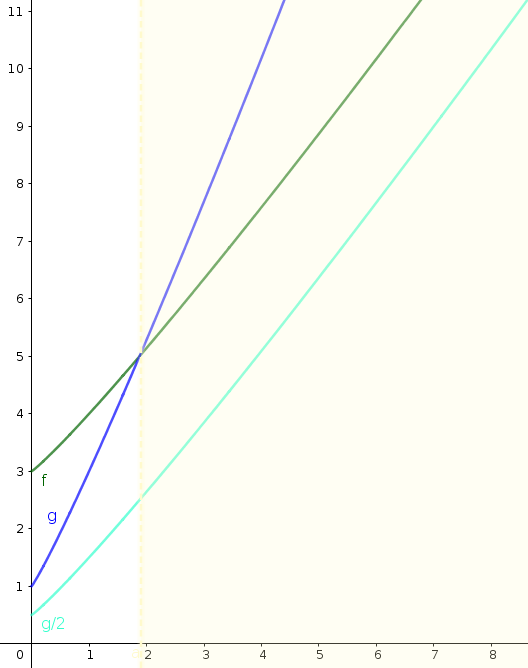
\includegraphics[height=8 cm]{./images/complejidad1.png}
\end{frame}
\end{comment}


\begin{comment}
\begin{frame}{}
    \begin{alertblock}{Otras propiedades}
      \begin{enumerate}
          \item $f \sim g \iff f(n) \in \Theta(g(n))$ es una relación de equivalencia.
          \item $\Theta(f(n)+g(n)) = \Theta(\max\{f(n),g(n)\})$.
          \item $\Theta(cf(n)) = \Theta(f(n)), c \in \R^+$.
          \item Algunas clases destacadas:
          \[ \Theta(1) \subsetneq \Theta(\log(n)) \subsetneq \Theta(n) \subsetneq \Theta(n\log(n)) \subsetneq \Theta(n^2) .\]
      \end{enumerate}
    \end{alertblock}
    
    Dado un algoritmo que calcule la transformada de Fourier discreta de tamaño $N$, medimos su tiempo, $T(N)$. Queremos clasificar $T$ por su complejidad.
\end{frame}
\end{comment}

\subsection{La Transformada de Fourier Rápida}

\begin{frame}{Motivación: El producto de polinomios}
    El producto de polinomios es una operación muy común en numerosas aplicaciones.
    \begin{tcolorbox}[colback=ChetwodeBlue!10,colframe=ChetwodeBlue!60]
  \begin{center}
    {\color{TurkishRose}Multiplicación clásica: $\Theta(N^2)$ operaciones.}
    
    {\color{TurkishRose} (¡Sumar es solo $\Theta(N)$!)}
  \end{center}
  \end{tcolorbox}
  
  Sean $F(z) = \sum_{k=0}^{N-1}a_kz^k$, $G(z) = \sum_{k=0}^{N-1}b_kz^k$.
  $a \equiv (a_0,\dots,a_{N-1},0,\dots,0)$, $b \equiv (b_0,\dots,b_{N-1},0,\dots,0)$.
  
  $(FG)(z) = \sum_{k=0}^{2N-2} c_kz^k$, donde $c_k = \sum_{j=0}^{k}a_jb_{k-j} = (a \ast b)(k)$.
  
  \begin{tcolorbox}[colback=ChetwodeBlue!10,colframe=ChetwodeBlue!60]
  \begin{center}
    {\color{TurkishRose} $coefs(PQ) = coefs(P) \ast coefs(Q)$}
  \end{center}
  \end{tcolorbox}
  
  ¿Convolución rápida? $f \ast g = D^{-1}(Df \cdot Dg)$.
  
\end{frame}

\begin{frame}{Una primera aproximación}

\begin{block}{Polinomios asociados a funciones discretas}
    Sea $f\colon \Z_N \to \C$. Definimos su polinomio asociado $P_f\colon \C \to \C$ por
    \[ P_f(z) = \sum_{k=0}^{N-1}f(k)z^k. \]
\end{block}
 \onslide<2->
La transformada de Fourier de $f$ se obtiene al evaluar $P_f$ en las raíces $N$-ésimas de la unidad.

 \onslide<3->
\begin{alertblock}{Idea: Calcular la transformada evaluando.}
    \begin{enumerate}
        \item Coste de una evaluación: $\Theta(N)$ (Algoritmo de Horner).
        \item Tenemos que evaluar $P_f$ en $N$ puntos distintos.
    \end{enumerate}
    Por tanto, el coste del algoritmo es de $\Theta(N^2)$.
\end{alertblock}

 \onslide<4->
¿Podemos mejorarlo? \textbf{Divide y vencerás}.

\end{frame}

\begin{frame}{Buscando una transformada rápida}
    Supongamos $N = 2^l$, con $l \in \N$, $f \colon \Z_N \to \C$.
    \[ P(z) = P_f(z) = f(0)+f(1)z+\dots+f(N-1)z^{N-1}. \]
    \onslide<2->
    Descomponemos $f$ en dos polinomios de tamaño $N/2$.
    \begin{align*}
        P_0(z) &= f(0) + f(2)z + f(4)z^2 + \dots + f(N-2)z^{N/2-1} \\
        P_1(z) &= f(1) + f(3)z + f(5)z^2 + \dots + f(N-1)z^{N/2-1}
    \end{align*}
    \onslide<3->
    \begin{tcolorbox}[colback=ChetwodeBlue!10,colframe=ChetwodeBlue!60]
        \[ P(z) = P_0(z^2) + zP_1(z^2) \]
    \end{tcolorbox}
    
    \onslide<4->
    Evaluamos en las raíces $N$-ésimas de la unidad.
    \[ P(\zeta_N^{-k}) = P_0(\zeta_N^{-2k})+\zeta_N^{-k}P_1(\zeta_N^{-2k}) = P_0(\zeta_{N/2}^{-k})+\zeta_{N}^{-k}P_1(\zeta_{N/2}^{-k}) \]
\end{frame}

\begin{frame}{Buscando una transformada rápida}
    Hemos obtenido transformadas de Fourier de dimensión $N/2$.
    \begin{align*}
        D_Nf(k) &= D_{N/2}f_0(k) + \zeta_{N}^{-k}D_{N/2}f_1(k) \\
        D_Nf(k+N/2) &= D_{N/2}f_0(k) - \zeta_{N}^{-k}D_{N/2}f_1(k) \\
        k&=0, \dots,N/2-1
    \end{align*}
    \onslide<2->
    Podemos repetir el proceso hasta llegar a $N=1$, donde $D_1f(0) = P_f(1) = f(0)$. Tenemos por tanto un algoritmo recursivo.
    
    \onslide<3->
    \begin{alertblock}{Eficiencia del algoritmo}
        Sea $T(N)$ el tiempo del algoritmo para un tamaño $N$.
        \begin{enumerate}
             
            \item Operaciones sobre vectores: $cN$, $c$ cte.
         
            \item Dos llamadas recursivas de tamaño $N/2$.
        \end{enumerate}

        Por tanto, $T(N) = 2T(N/2) + cN$.
        Esta ecuación tiene como solución $T(N) = aN + bN \log_2 N \in \Theta(N \log N)$.
    \end{alertblock}
\end{frame}

\begin{frame}{Comparación de transformadas rápidas}
    \centering
    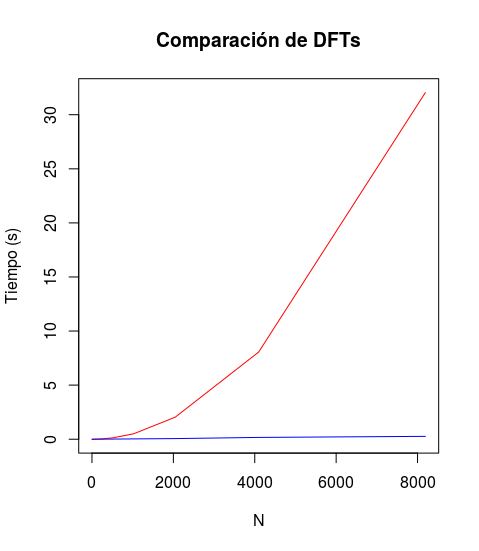
\includegraphics[height=6.5 cm]{./images/dft_comp.png}
    \textbf{¡Hemos encontrado una transformada rápida!}
\end{frame}

\begin{comment}
\begin{frame}{Observaciones}
    \begin{enumerate}
        \item El mismo algoritmo es aplicable para la transformada inversa.
        \item Necesario que $N$ sea una potencia de dos. Sin embargo, estos valores son muy útiles en algunas aplicaciones.
        \item Se conocen distintos algoritmos cuando $N$ no es potencia de dos.
        
    \end{enumerate}
\end{frame}
\end{comment}

\subsection{Otras transformadas rápidas}

\begin{comment}
\begin{frame}{Convolución}

    Sean $N, M, m \in \N$ tales que $M = 2^m$ y $2^{m-1} \ge N > 2^{m-2}$. Dadas $g,h\colon \Z_N \to \C$, podemos extenderlas a $G,H \colon \Z_M \to \C$ de forma que $(g \ast h)(n) = (G \ast H)(n)$ para $n = 0,\dots,N-1$.
    
    \begin{alertblock}{Eficiencia de la convolución}
        Sabemos que $g \ast h = G \ast H = D^{-1}(DG \cdot DH)$ en $\{0,\dots,N-1\}$, luego la convolución se reduce a tres transformadas rápidas, esto es, $\Theta(M \log M) = \Theta(N \log N)$.
    \end{alertblock}
    
    \begin{block}{Producto de polinomios}
        Sean $P,Q \colon \C \to \C$ polinomios de grado menor que $N$. Entonces, se verifica que
        \[ coefs(PQ) = coefs(P)\ast coefs(Q), \]
        donde $coefs(F)$ es el vector con los $2N-1$ primeros coeficientes del polinomio $F$, extendido por ceros. Por tanto, podemos multiplicar polinomios en $\Theta(N \log N)$.
    \end{block}

\end{frame}
\end{comment}

\begin{frame}{}

\begin{block}{Transformada de Bluestein}
    \textbf{La transformada es una convolución}
    \[Df(n) = \zeta^{-n^2/2}(g \ast h)(n),\]
    donde $g(n) = f(n) \zeta^{-n^2/2}$ y $h(n) = \zeta^{n^2/2}$, $n \in \{0,\dots,N-1\}$.
\end{block}

\onslide<2->
\begin{block}{Transformada bidimensional}
    \[ Df(n_1,n_2) = \sum_{k_1=0}^{N_1-1}\left(\sum_{k_2=0}^{N_2-1} f(k_1,k_2)\zeta_{N_2}^{-n_2k_2}\right)\zeta_{N_1}^{-n_1k_1} \]
    
    \begin{enumerate}
        \item $N_1$ transformadas de dimensión $N_2$: $f_{n_1}(n_2) = f(n_1,n_2)$.
        \item $N_2$ transformadas de dimensión $N_1$: $(D_{N_2}f_0(n_2),\dots,D_{N_2}f_{N_1-1}(n_2))$.
        \[ N_1 \Theta(N_2\log N_2) + N_2 \Theta(N_1 \log N_1) = \Theta(N_1N_2 \log(N_1N_2)) \]
    \end{enumerate}

\end{block}



\end{frame}

\begin{comment}
\section{Motivación}
	
\subsection{Deep learning}
	
\begin{frame}{¿Dónde se usa Deep Learning? - {\color{TurkishRose}\textbf{Pattern Recognition}}}

  \begin{columns}
    \column{0.53\textwidth} \vspace*{-4mm}
    \begin{figure}[H]
      \centering
      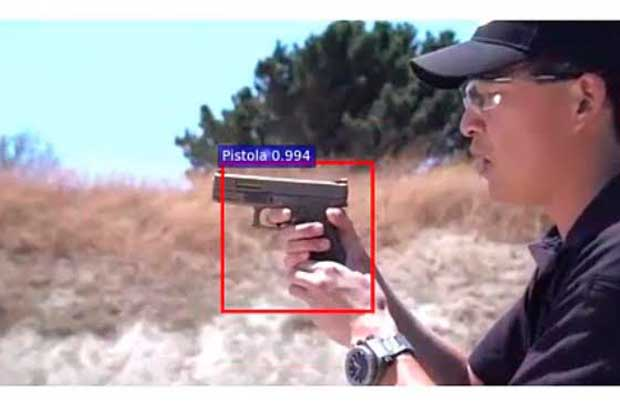
\includegraphics[width=\textwidth]{./images/detector-pistola-ugr.jpg}
    \end{figure}
    \vspace*{-8mm}
    \begin{figure}[H]
      \centering
      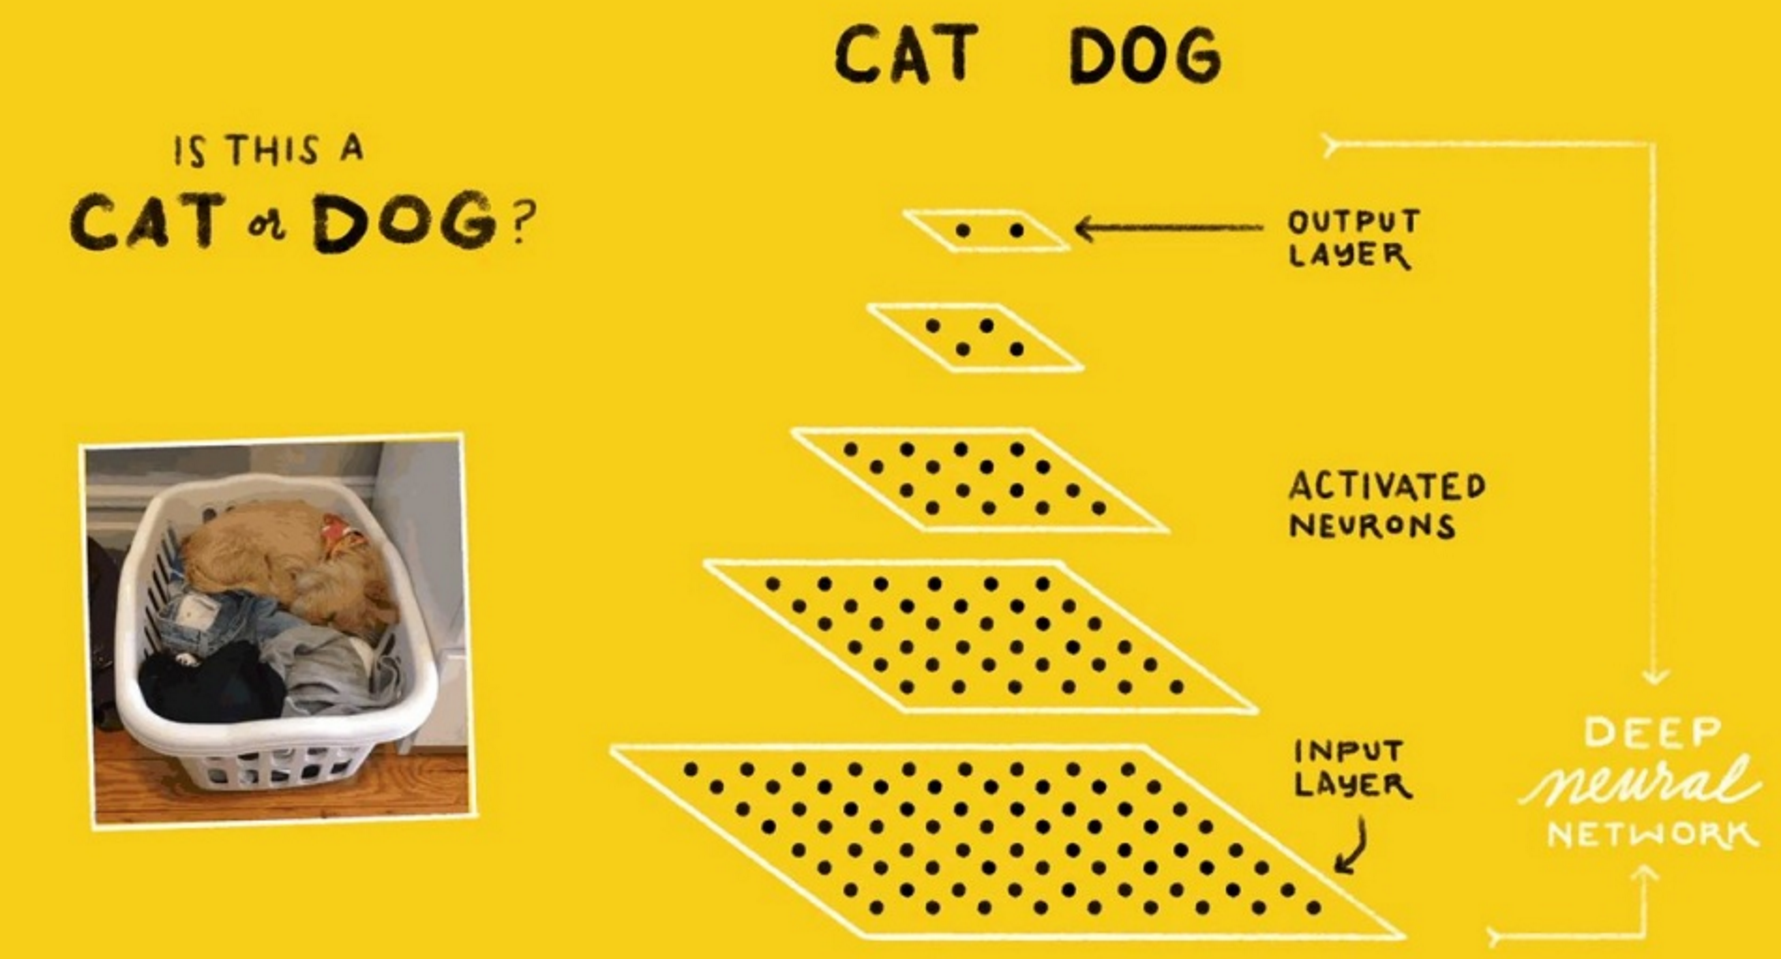
\includegraphics[width=\textwidth]{./images/cat-dog.png}
    \end{figure}
			
    \column{0.53\textwidth} \vspace*{-3.5mm}
    \begin{figure}[H]
      \centering
      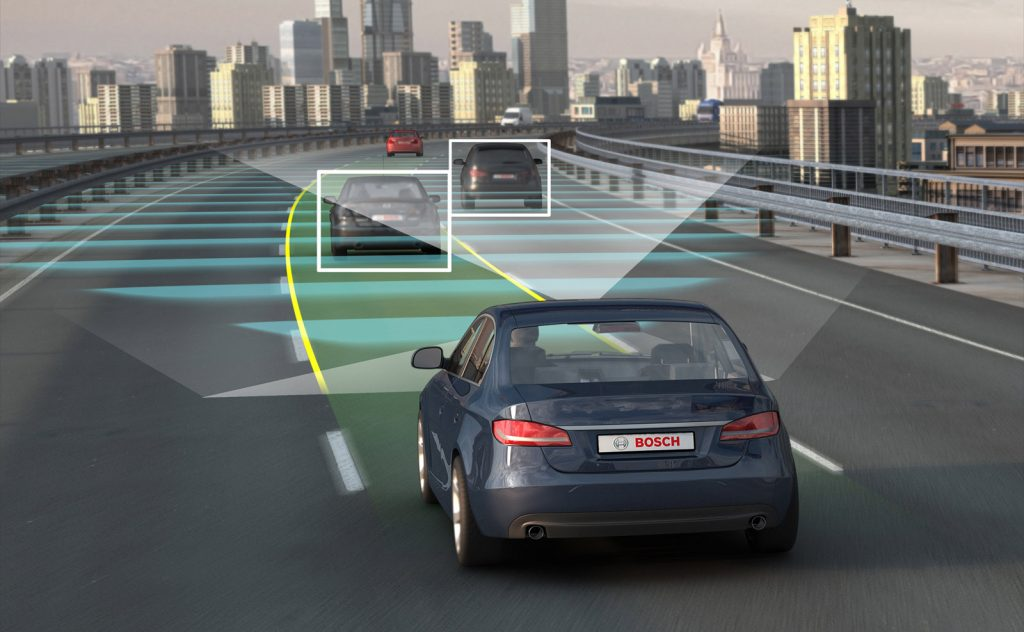
\includegraphics[width=\textwidth]{./images/autonomous-car.jpg}
    \end{figure}
    \vspace*{-8mm}
    \begin{figure}[H]
      \centering
      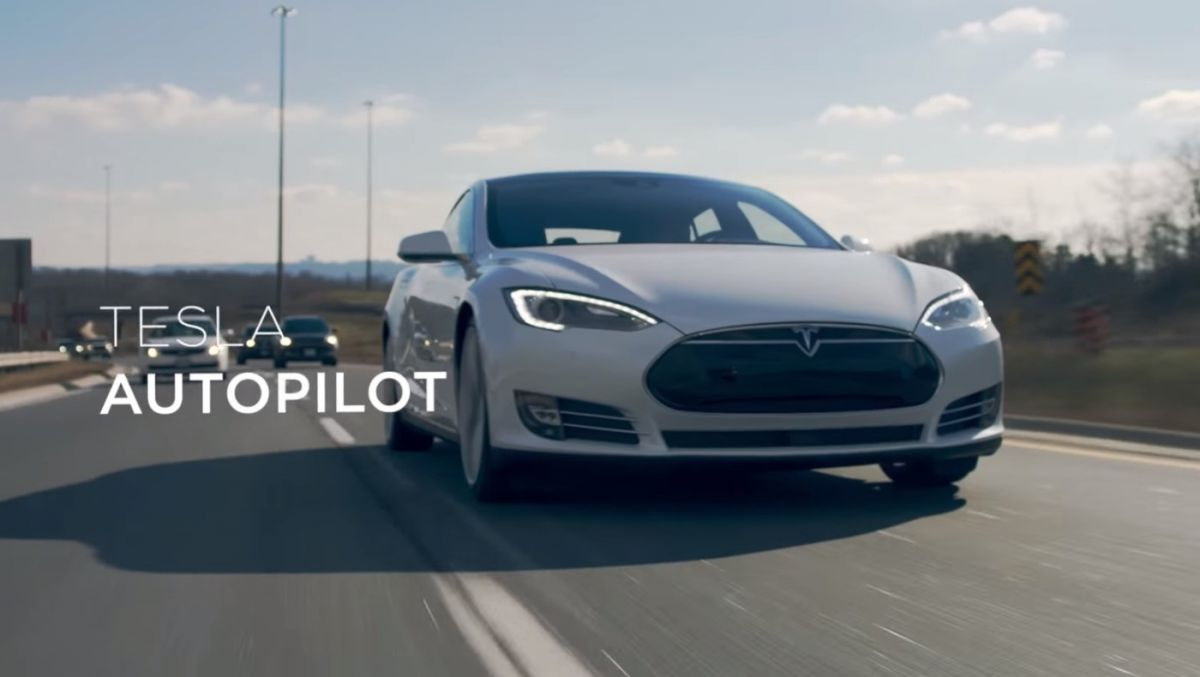
\includegraphics[width=\textwidth]{./images/tesla.jpg}
    \end{figure}
  \end{columns}
\end{frame}
		
\begin{frame}{¿Dónde usa Google Deep Learning?}
  \begin{columns}
    \column{0.55\textwidth}
    \begin{figure}[H]
      \centering
      
\includegraphics[width=0.5\textwidth]{./images/deepmind-logo.jpg}
    \end{figure}
    \vspace*{-7mm}
    \begin{figure}[H]
      \centering
      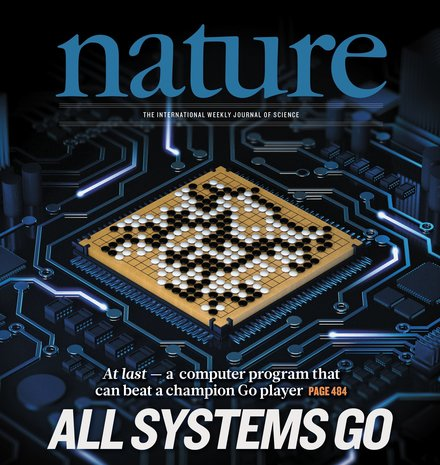
\includegraphics[width=0.8\textwidth]{./images/nature.jpg}
    \end{figure}
			
    \column{0.4\textwidth}
    \begin{center}
      {\color{TurkishRose}\textbf{Aplicaciones}}
    \end{center}
    \fontsize{10}{8}\selectfont
    \begin{itemize}
    \item \textbf{RankBrain} \\ \vspace*{2mm}(Search Queries)
    \item \textbf{Google Translator}
    \item \textbf{Google Photos}
    \item \textbf{Deep Mind Health}
    \item \textbf{Google Street View} \\ \vspace*{2mm} (obtención de textos)
    \item \textbf{Predicción} \\ \vspace*{2mm} (Enfriamiento de CPDs)
    \item \textbf{¡Muchos otros!}
    \end{itemize}
  \end{columns}
\end{frame}

\begin{frame}{Deep Neural Networks - {\color{TurkishRose}\textbf{Machine Learning}}}
  % \begin{center}
  %   \textbf{Clasificación y Predicción}
  % \end{center}
  % \begin{columns}
  %   \column{0.8\textwidth} \vspace*{-0mm}
  \vspace{-1mm}
  \begin{center}
    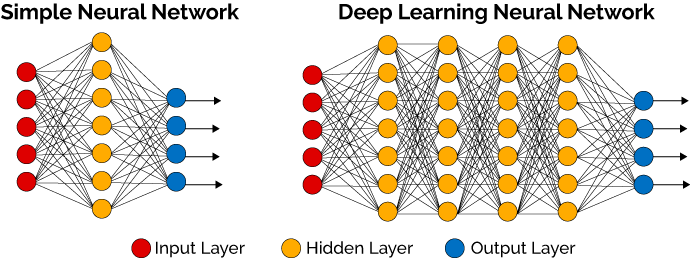
\includegraphics[width=0.8\textwidth]{./images/neural-network.png}
  \end{center}
  % \column{0.35\textwidth} \vspace*{-2cm}
  % \begin{tcolorbox}[colback=ChetwodeBlue!10,colframe=ChetwodeBlue!60]
  %   \begin{center}
  %     \fontsize{8}{8}\selectfont
  %     \begin{enumerate}
  %     \item \textbf{Regresión}
  %     \item \textbf{Clasificación}
  %     \end{enumerate}
  %   \end{center}
  % \end{tcolorbox}
  % \end{columns}
  \begin{columns}
    \column{0.5\textwidth} \vspace*{-8mm}
    \begin{figure}[H]
      \centering
      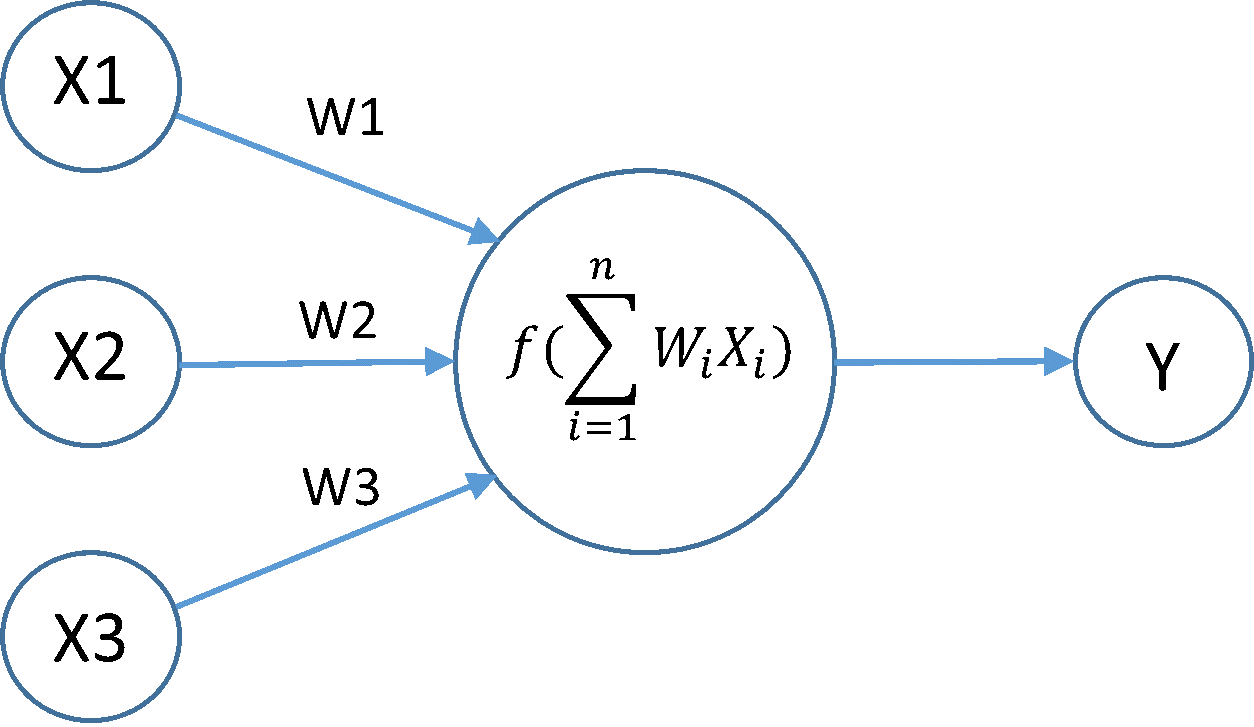
\includegraphics[width=\textwidth]{./images/neuron.png}
    \end{figure}

    \column{0.58\textwidth} \vspace{-2mm}
    \begin{tcolorbox}[colback=ChetwodeBlue!10,colframe=ChetwodeBlue!60]
      \begin{center}
        \fontsize{9}{5}\selectfont {\color{TurkishRose}\textbf{Operaciones habituales}}
    
        \begin{enumerate}
        \item Productos entre tensores, i.e., \vspace*{-2mm}
          \begin{equation*}
            \langle x, y \rangle = \sum_{i = 1}^{n} x_i y_i            
          \end{equation*}
          \vspace*{-4mm}
        \item Funciones de activación
        \end{enumerate}
      \end{center}
    \end{tcolorbox}
  \end{columns}
  \vspace{-2mm}
  \begin{center}
    \fontsize{9}{5}\selectfont \textbf{¡Hay que realizar múltiples operaciones matriciales!}
  \end{center}
\end{frame}

\section{Tensor Processing Unit}

\subsection{Funcionamiento}

\begin{frame}{¿Qué es una TPU?}
  \vspace*{-3mm}
  \begin{center}
    {\color{TurkishRose} \textbf{Application-Specific Integrated Circuit (ASIC) \\ for neural
        networks computations}}
  \end{center}
  \begin{columns}
    \column{0.6\textwidth}
    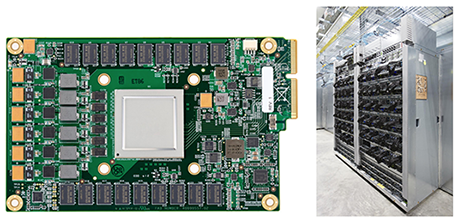
\includegraphics[width=\textwidth]{./images/tpu-chip.png}
    \column{0.55\textwidth}
      
    \begin{enumerate}
    \item Arquitectura de 8 bits
    \item Multiplicaciones Matriciales
    \item Complex Instruction Set Computer (CISC)
    \item Arquitectura ``Systolic Array''
    \end{enumerate}
  \end{columns}
  \vspace*{2mm}
  \begin{tcolorbox}[colback=ChetwodeBlue!10,colframe=ChetwodeBlue!60]
    \begin{columns}
      \column{0.87\textwidth} \fontsize{10}{7}\selectfont ``TPU design encapsulates the essence of
      neural network calculation, and can be programmed for a wide variety of neural network
      models.''  \column{0.13\textwidth}
      
\includegraphics[width=\textwidth]{./images/logo-google.png}
    \end{columns}
  \end{tcolorbox}
\end{frame}

\begin{frame}{Arquitectura de 8 bits: {\color{TurkishRose}Quantization}}
  \vspace*{-2.5mm}
  \begin{center}
    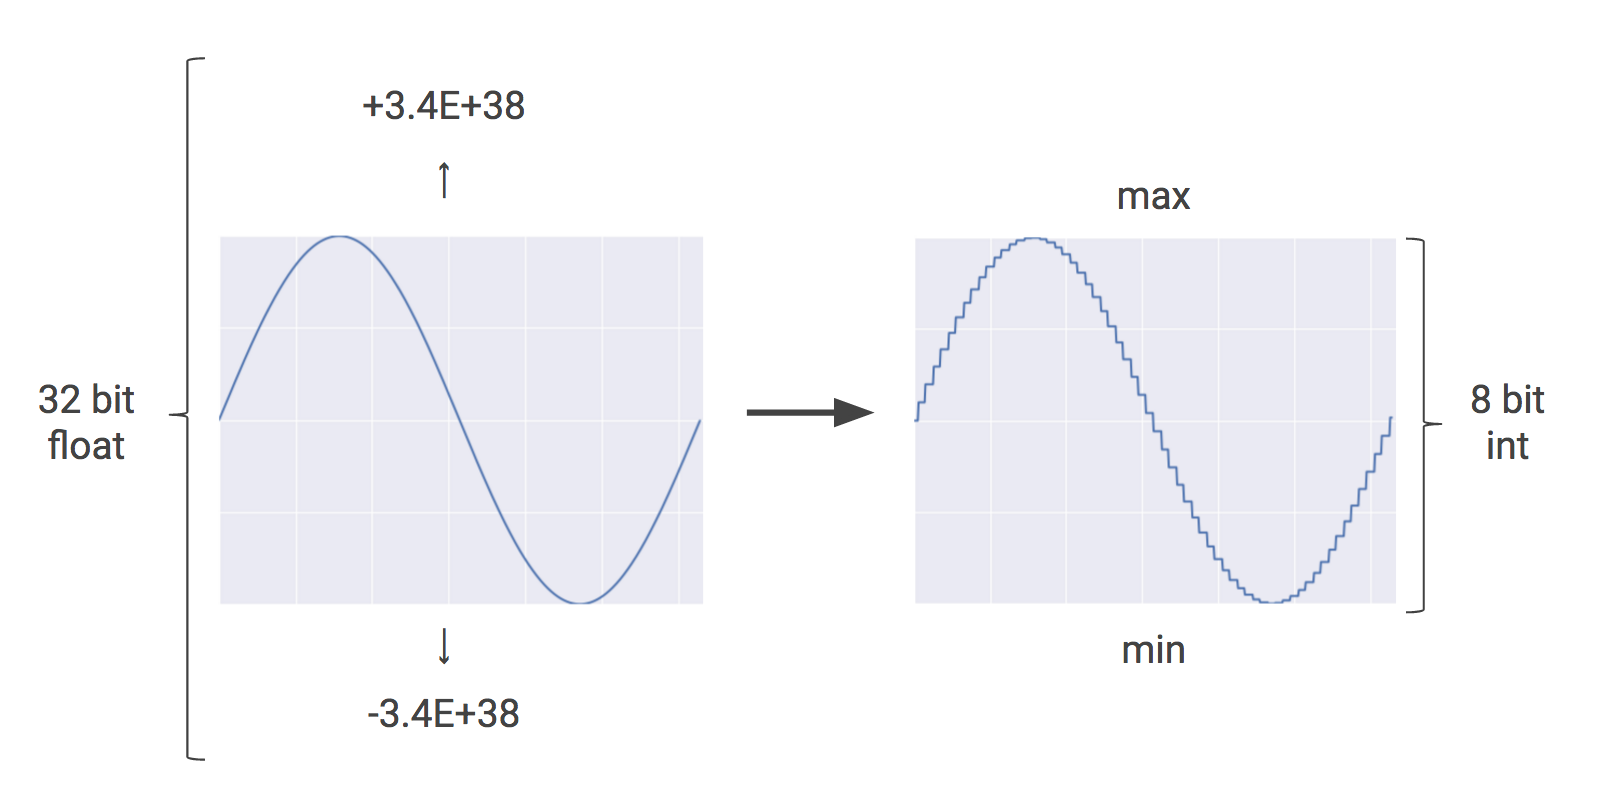
\includegraphics[width=0.78\textwidth]{./images/quantization.png}
  \end{center}
  \vspace*{-4mm}
  \begin{tcolorbox}[colback=ChetwodeBlue!10,colframe=ChetwodeBlue!60]
    \begin{center}
      \fontsize{8}{5}\selectfont
      \begin{itemize}
      \item Las redes neuronales no se ven afectadas por la falta de precisión.
        \[ x \in [a, b] \Rightarrow x = (b-a) \frac{n}{255} + a \text{ con } n \in [0,255]\]
      \item La cuantización de $x$ en $[a,b]$ es el redondeo de $n$.
      \end{itemize}
      \fontsize{10}{10}\selectfont
      \vspace{0.5mm}
     {\color{TurkishRose} \textbf{ ¡Las operaciones no son en coma flotante!  }}
      \vspace{-1mm}
    \end{center}
  \end{tcolorbox}
\end{frame}

\begin{frame}{Complex Instruction Set Computer}
  \begin{table}[H]
    \centering
    \begin{tabular}{ll}
      \toprule
      \textbf{Instrucción TPU} & \textbf{Función} \\
      \toprule
      Read\_Host\_Memory & Read data from memory \\
      Read\_Weights & Read weights from memory  \\
      MatrixMultiply/Convolve & Multiply or convolve with the \\
                               & data and weights, accumulate \\
                               & the results \\ 
      Activate & Apply activation functions  \\
      Write\_Host\_Memory & Write result to memory  \\
      \bottomrule
    \end{tabular}
  \end{table}
  \begin{center}
    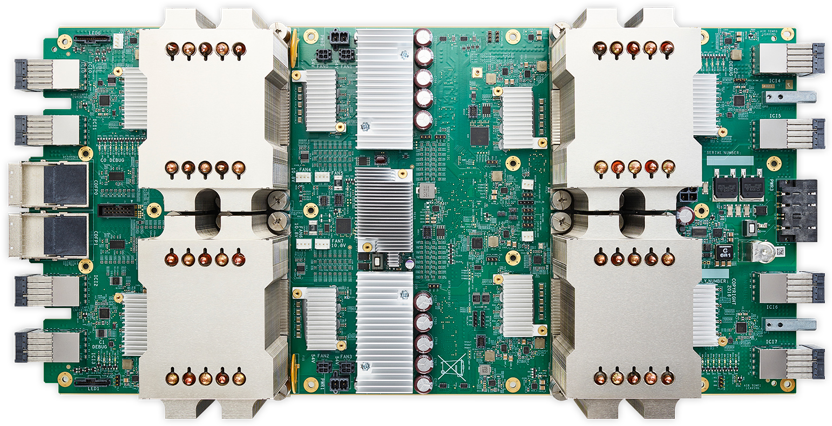
\includegraphics[width=0.4\textwidth]{./images/tpu-chip-2.png}
  \end{center}
  
\end{frame}

\begin{frame}{Arquitectura Systolic Array}
  \vspace*{-2mm}
  \begin{center}
    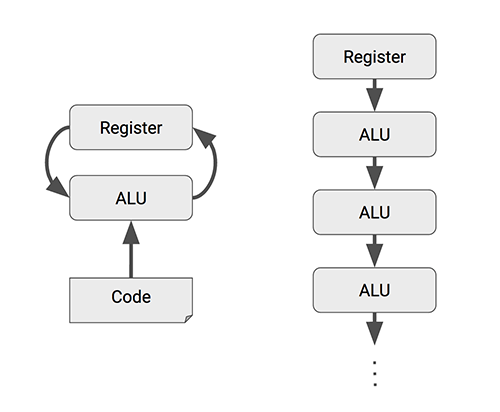
\includegraphics[width=0.75\textwidth]{./images/systolic-array.png}
    \vspace*{-2mm}
    
    {\color{TurkishRose}\textbf{¡No necesitan memorias caché!}}
  \end{center}
\end{frame}

\subsection{API}

\begin{frame}{TPU - Application Programming Interface}
  \begin{columns}
    \column{0.4\textwidth}
    \begin{center}
      
\includegraphics[width=\textwidth]{./images/tensor-flow.png}
    
       {\Large\color{ChetwodeBlue}\textbf{Tensor Flow}}
    \end{center}
    \column{0.6\textwidth}
    \begin{center}
      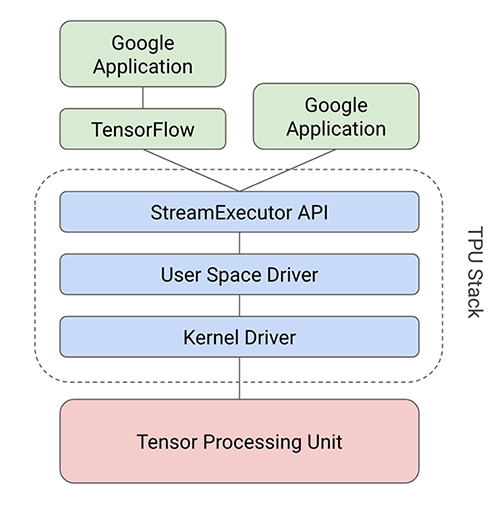
\includegraphics[width=\textwidth]{./images/tpu-tensor-flow.png}
    \end{center}

  \end{columns}
\end{frame}

\end{comment}

\begin{comment}
\section{Comparación}

\subsection{Cómputo}

\begin{frame}
  \frametitle{Capacidad de cómputo}

  \begin{center}
    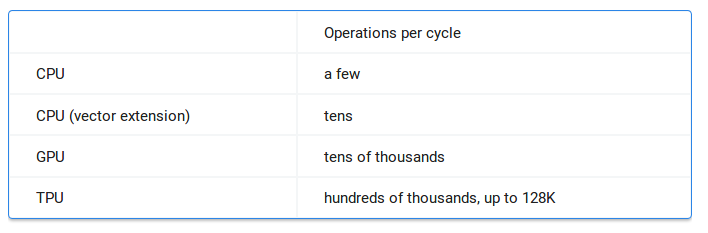
\includegraphics[width=\textwidth]{./images/operaciones.png}
  \end{center}
  \vspace*{-2mm}
  {\fontsize{9}{5}\selectfont \textbf{Nota:} Google usa Nvidia Tesla K80 (2014)}
  \vspace*{2mm}
  \begin{tcolorbox}[colback=ChetwodeBlue!10,colframe=ChetwodeBlue!60]
    \begin{center}
     {\color{TurkishRose} \textbf{Características de una TPU}}      
    \end{center}
    \vspace{-5mm}
    \fontsize{9}{5}\selectfont
    \begin{itemize}
    \item 65.536 operaciones / ciclo  con enteros de 8 bits 
    \item TPU funciona a 700MHz
    \item 92 Teraops por segundo
    \end{itemize}
  \end{tcolorbox}
\end{frame}

\begin{frame}{Capacidad de Cómputo}
  \begin{center}
    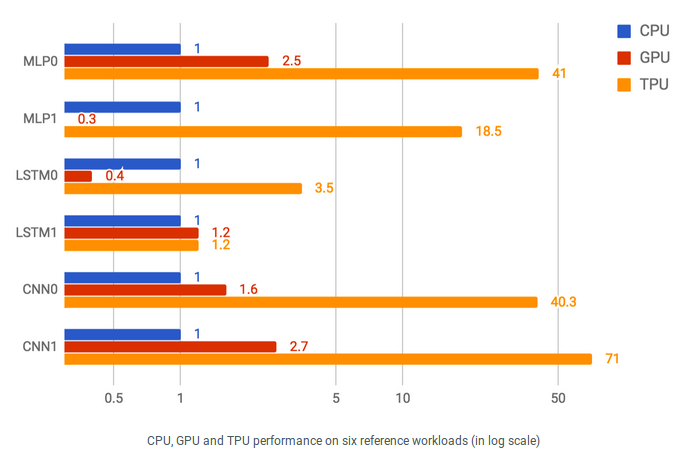
\includegraphics[width=0.9\textwidth]{./images/performance-2.png}
  \end{center}
\end{frame}

\subsection{Rendimiento}

\begin{frame}{Capacidad de Cómputo / Potencia Energética}
  \begin{center}
    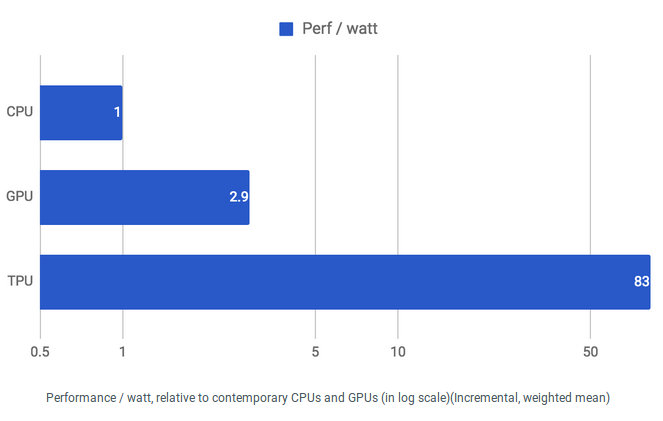
\includegraphics[width=\textwidth]{./images/tpu-wat-2.png}
  \end{center}
\end{frame}

\end{comment}

%%%%%%%%%%%%%%%%%%%%%%%%%%%%%%%%%%%%%%%%%%%%%%%%%%%%%%%%%%%%%%%%%%%%%%%%%%%%%%%%%%%%%
% QUANTUM COMPUTING
%%%%%%%%%%%%%%%%%%%%%%%%%%%%%%%%%%%%%%%%%%%%%%%%%%%%%%%%%%%%%%%%%%%%%%%%%%%%%%%%%%%%%

\section{Quantum Computing}

\subsection{¿Para qué sirve Quantum Computing?}

\begin{frame}{Quantum Computing no es ciencia ficción}

  \begin{columns}
    \column{0.5\textwidth}
    \begin{center}
    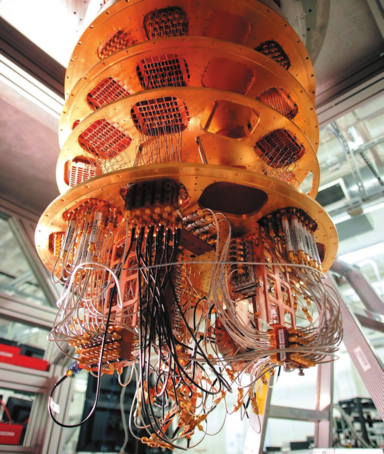
\includegraphics[width=0.85\textwidth]{./images/google-cryostats-2.png}

    {\large\color{ChetwodeBlue}\textbf{Google}}
    \end{center}
    \column{0.5\textwidth}
    \begin{center}
    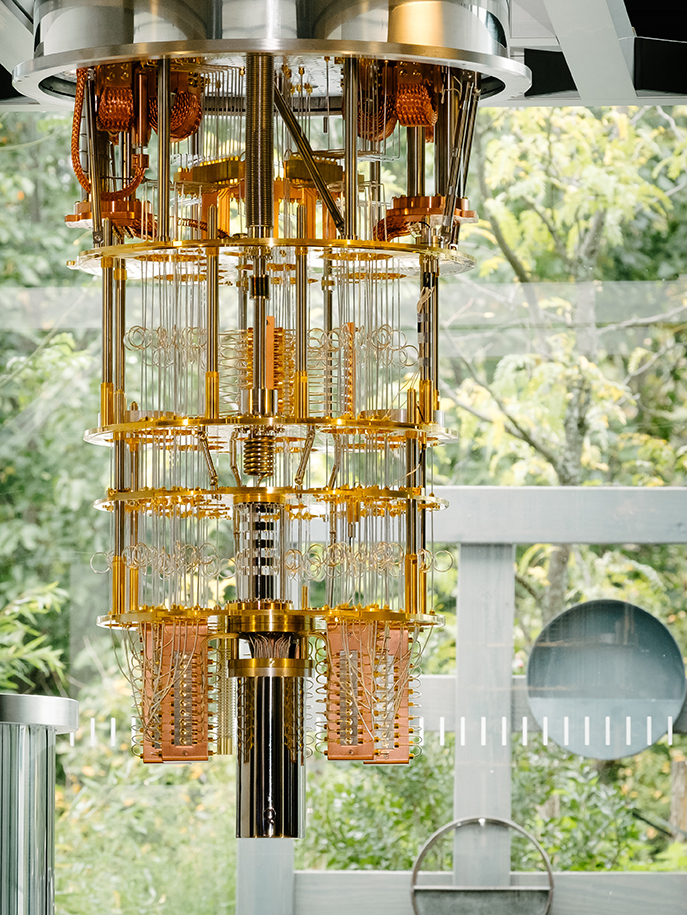
\includegraphics[width=0.78\textwidth]{./images/ibm-50q.jpg}

    {\large\color{ChetwodeBlue}\textbf{IBM}}
    \end{center}
  \end{columns}
  \begin{tcolorbox}[colback=ChetwodeBlue!10,colframe=ChetwodeBlue!60]
    %\fontsize{9}{5}\selectfont
    %Múltiples empresas y centros de investigación están desarrollando ordenadores cuánticos.
    \begin{center}
      {\large\color{TurkishRose}\textbf{¡Ya existen ordenadores cuánticos!}}
    \end{center}
  \end{tcolorbox}
%    \begin{center}
%      {\large\color{TurkishRose}\textbf{Criogenizadores}}
%    \end{center}
\end{frame}

\begin{frame}
  \begin{center}
    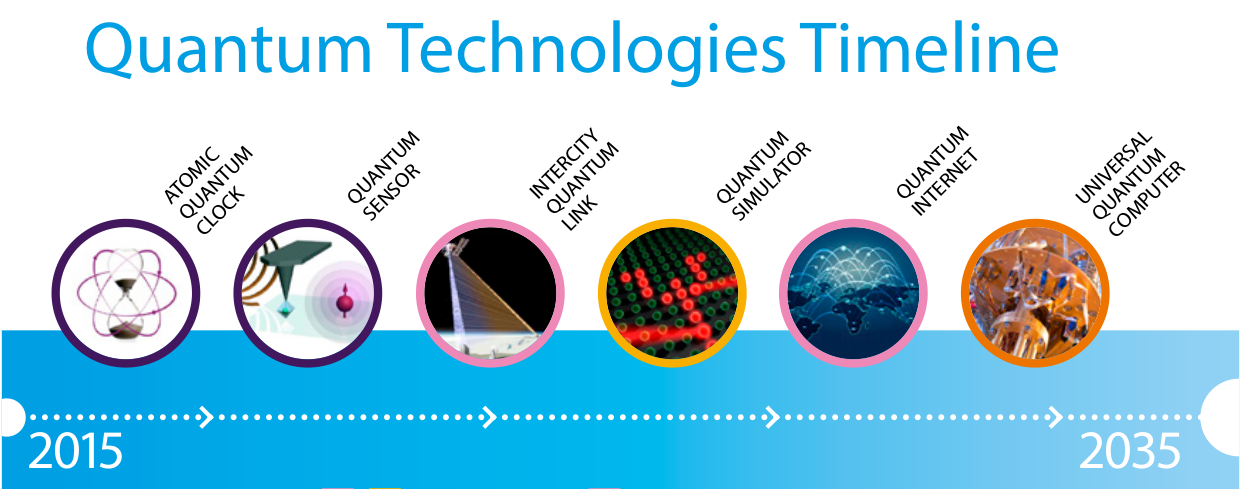
\includegraphics[width=\textwidth]{./images/quantum-prediction.png}
  \end{center}
  
  \begin{tcolorbox}[colback=ChetwodeBlue!10,colframe=ChetwodeBlue!60]
    \textbf{Investigación en Quantum Computing:}
    \begin{enumerate}
    \item Desarrollo y construcción de ordenadores cuánticos -- {\color{TurkishRose}\textbf{Física e ingeniería} \faWarning}
    \item ¿Qué puede calcular un ordenador cuántico de forma eficiente? -- {\color{TurkishRose}\textbf{Informática Teórica $\subset$ Matemáticas} \faHeart}
    \end{enumerate}
  \end{tcolorbox}

\end{frame}

\begin{frame}{¿Por qué es importante?}

 \begin{theorem}
   Todo algoritmo clásico puede ser simulado con igual eficiencia en un ordenador cuántico.
  \end{theorem}
  
  \begin{tcolorbox}[colback=ChetwodeBlue!10,colframe=ChetwodeBlue!60]
    %\fontsize{9}{5}\selectfont
    %Múltiples empresas y centros de investigación están desarrollando ordenadores cuánticos.
    \begin{center}
      {\large\color{TurkishRose}\textbf{Se cree que la computación cuántica es mejor teóricamente que la clásica.}}
    \end{center}
  \end{tcolorbox}

\begin{block}{Problema de la factorización de enteros}
   Dado $N \in \mathbb{Z}$, calcula la descomposición en factores primos de $N$. 
   
{\color{TurkishRose}El mejor algoritmo clásico conocido realiza $\theta(\exp(n^{1/3} \log^{2/3} n))$ operaciones, donde $n = \log_2 N$.}
\end{block}

%\begin{theorem}[Criba general del cuerpo de números]
%\end{theorem}

\begin{theorem}[Algoritmo de Shor]
Existe un algoritmo cuántico para factorizar números enteros que utiliza como mucho $\theta(n^4)$ ``operaciones cuánticas'', donde $n = \log_2 N$.
\end{theorem}
\end{frame}

\begin{frame}{Teoría de la Complejidad Cuántica}

  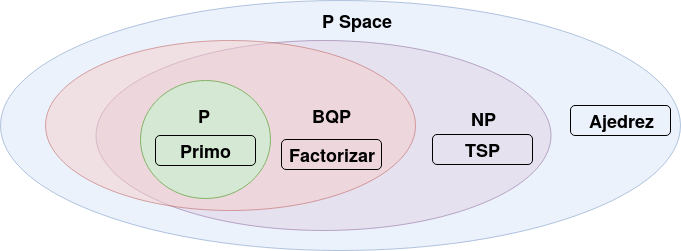
\includegraphics[width=\textwidth]{./images/complexity-zoo.png}

  \begin{tcolorbox}[colback=ChetwodeBlue!10,colframe=ChetwodeBlue!60]
    %\fontsize{9}{5}\selectfont
    %Múltiples empresas y centros de investigación están desarrollando ordenadores cuánticos.
    \begin{center}
      {\color{TurkishRose}\textbf{¡La criptografía actual se basa en que no podemos factorizar un número en un tiempo razonable!}}
    \end{center}
    Tiempo necesario para factorizar un entero de 728 bits:
    \begin{enumerate}
        \item Ordenador clásico: {\color{TurkishRose}\textbf{2000 años}}.
        \item Ordenador cuántico: \textbf{segundos}.
    \end{enumerate}
  \end{tcolorbox}

\end{frame}

\subsection{¿Cómo calcula un ordenador cuántico?}

\begin{frame}{La unidad de memoria cuántica: el qubit}

\begin{center}
{\color{TurkishRose}¡Es un caso particular de la mecánica cuántica!}
\end{center}

\begin{definition}
    \fontsize{10}{5}\selectfont

\begin{enumerate}
    \item Un \textbf{qubit} es un sistema cuántico cuyo \textbf{espacio de estados} es $\mathbb{C}^2$. Denotamos por $\{\ket{0}, \ket{1}\}$ a una base ortonormal de este espacio.
    \item El \textbf{estado del qubit} es un vector unitario del espacio de estados, esto es, $\ket{\Psi} = a \ket{0} + b \ket{1}$ con $|a|^2 + |b|^2 = 1$ y $a,b \in \mathbb{C}$.
    \item Un ordenador cuántico cambia el vector de estado de un qubit aplicando isometrías de $\mathbb{C}^2$, denominadas \textbf{operaciones cuánticas}.
    \item Un qubit se puede \textbf{medir}, dando dos posibles resultados $0$ y $1$, con probabilidad $|a|^2$ y $|b|^2$ respectivamente. El nuevo estado del qubit es $\ket{0}$ si el resultado fue $0$ y $\ket{1}$ en caso contrario.
\end{enumerate}
\end{definition}
  \begin{tcolorbox}[colback=ChetwodeBlue!10,colframe=ChetwodeBlue!60]
  \begin{center}
    {\color{TurkishRose}¡Un bit clásico solo toma dos valores $0$ y $1$!}
  \end{center}
  \end{tcolorbox}
\end{frame}

\begin{frame}
%  \begin{tcolorbox}[colback=ChetwodeBlue!10,colframe=ChetwodeBlue!60]
%    \fontsize{9}{5}\selectfont
%    ``La única diferencia entre un mundo regido por la probabilidad clásica y el mundo de la mecánica cuántica es que, por alguna razón, las probabilidades deberían ser negativas'' -- \linebreak Richard Feynman, premio Nobel de física en 1965.
%  \end{tcolorbox}    
  
  \begin{definition}[Registro de qubits]
    \fontsize{10}{5}\selectfont
    \begin{enumerate}
  	  \item Un \textbf{registro de qubits} es un sistema cuántico compuesto por $n$ qubits. El espacio de estados es el producto tensorial de los espacios, esto es, $\mathbb{C}^{N}$, con $N = 2^n$. Una base ortonormal es 
  	  \vspace{-3mm}
  	  \[\{\ket{j} : j \in \{0, \ldots, N-1\}\}.\] 
  	  \vspace{-5mm}
  	  \item El \textbf{estado del registro} es un vector unitario
  	  \vspace{-3mm}
  	  \[\ket{\Psi} = a_0 \ket{0} + a_1 \ket{1} + \cdots + a_{N-1} \ket{N-1}.\]
  	  \vspace{-5mm}
      \item Hay $N$ posibles resultados al \textbf{medir} el registro ($0, 1, \ldots, N-1$). La probabilidad de que el resultado sea $j$ es $|a_j|^2$, en cuyo caso el estado pasa a ser $\ket{j}$.
      \vspace{-2mm}
      \item Una \textbf{operación cuántica} es una isometría de $\mathbb{C}^N$ que actúa a lo sumo sobre $3$ qubits.
  	\end{enumerate}
  \end{definition}
  
  \begin{tcolorbox}[colback=ChetwodeBlue!10,colframe=ChetwodeBlue!60]
    \fontsize{10}{5}\selectfont
  Un \textbf{algoritmo cuántico} consiste en:
  \begin{enumerate}
  	 \item Aplicar una secuencia de operaciones cuánticas al registro.
  	 \item Medir el registro y devolver parte del resultado.
  \end{enumerate} 
  \end{tcolorbox}
\end{frame}

\subsection{Transformada de Fourier Cuántica}

\begin{frame}{La Transformada de Fourier Cuántica}
\begin{block}{Definición}
  La Transformada de Fourier de un estado  $\ket{f} = \sum_{j = 0}^{N-1} f(j) \ket{j}$ es
  \[ \ket{Df} = \frac{1}{\sqrt{N}}\sum_{j = 0}^{N-1} Df(j) \ket{j}. \]
  
  {\color{TurkishRose}El factor $1/\sqrt{N}$ hace que sea una isometría sobre $\mathbb{C}^N$}.
\end{block}

\begin{lemma}[Ecuación recurrente de la DFT]
\vspace{-7mm}
\begin{align*} \label{eq:qft}
    \ket{Df} & = \frac{1}{\sqrt{N}} \sum_{j = 0}^{N/2} \left(Df_0(j) +  \zeta^j Df_1(j)\right) \ket{0} \ket{j} \\
    & + \frac{1}{\sqrt{N}} \sum_{j = 0}^{N/2} \left(Df_0(j)  -  \zeta^j Df_1(j)\right) \ket{1} \ket{j}, %\\
\end{align*}
donde $f_0 = (f(0),f(2),\dots,f(N-2))$ y $f_1 = (f(1),f(3),\dots,f(N-1))$.
\end{lemma}
\end{frame}

\begin{frame}
    \fontsize{10}{5}\selectfont
\begin{lemma}[Transformada de Fourier cuántica]
  Existe un algoritmo cuántico que calcula la DFT de un registro con $n$ qubits utilizando $n^2-1 \in \theta(n^2)$ operaciones cuánticas.
\end{lemma}

Consideramos un registro con $m$ qubits ($M = 2^m)$ y estado
\begin{equation} \label{eq:period}
  \ket{\Psi} = \frac{1}{\sqrt{K}}\sum_{j = 0}^{K-1} \ket{r_0 + j r},
\end{equation}
  donde $K = \lfloor (M-r_0) / r \rfloor$. 
  %La Transformada de Fourier Cuántica puede aplicarse a \eqref{eq:period} para calcular el periodo $r$. Esta propiedad es clave para el desarrollo Algoritmo de Shor. 
  Aplicando la Transformada de Fourier Cuántica a este registro obtenemos
  \begin{equation} \label{eq:qft:period}
  \ket{D \Psi} = \frac{1}{\sqrt{K M}} \sum_{j = 0}^M \left(\sum_{l = 0}^{K-1} \zeta^{(r_o + l r) j} \right) \ket{j}.
  \end{equation}
 %El siguiente resultado determina una cota inferior de la probabilidad de obtener un múltiplo de $r$ al medir \eqref{eq:qft:period}, cuya demostración puede encontrarse en {\cite[Lemas 10.19 y 10.20]{arora}}.

\begin{theorem} \label{thm:qft}
  Existe $0 < c < 1$ tal que, para cualquier $m,r \in \mathbb{N}$ con $r < M = 2^m$, al medir \eqref{eq:qft:period} obtenemos, con probabilidad al menos $c/\log r$, un resultado de la forma $jr$ con $j \in \{0, \ldots, K-1\}$.
\end{theorem}

\end{frame}

\begin{frame}%{El algoritmo de Shor}

\begin{block}{Reducimos factorizar a calcular órdenes}
    \fontsize{10}{5}\selectfont
\begin{enumerate}
	\item Dado $x \in \left(\mathbb{Z} / N \mathbb{Z}\right)^\times$ aleatorio, calculamos el orden $r$ de $x$.
	\item $x^{r/2}$ es una raíz no trivial de $1$ módulo $N$ con probabiliad $1/2$.
	\item En tal caso, $\gcd(x^{r/2}+1, N)$ es un divisor no trivial de $N$.
	\end{enumerate}
\end{block}

\begin{theorem}[Algoritmo de Shor]
	El Algoritmo de Shor aplica $\theta(n^3)$ operaciones cuánticas para calcular el orden de $x \in \left(\mathbb{Z}/N\mathbb{Z}\right)$, donde $n = \log_2 N$.
\end{theorem}

Consiste en aplicar la transformada de Fourier cuántica a
\[\frac{1}{\sqrt{M}} \sum_{j = 0}^{M-1} \ket{j}\ket{x^j \pmod{N}},\]
estado que se calcula en $\theta(n^3)$.
\end{frame}
 
\usebackgroundtemplate{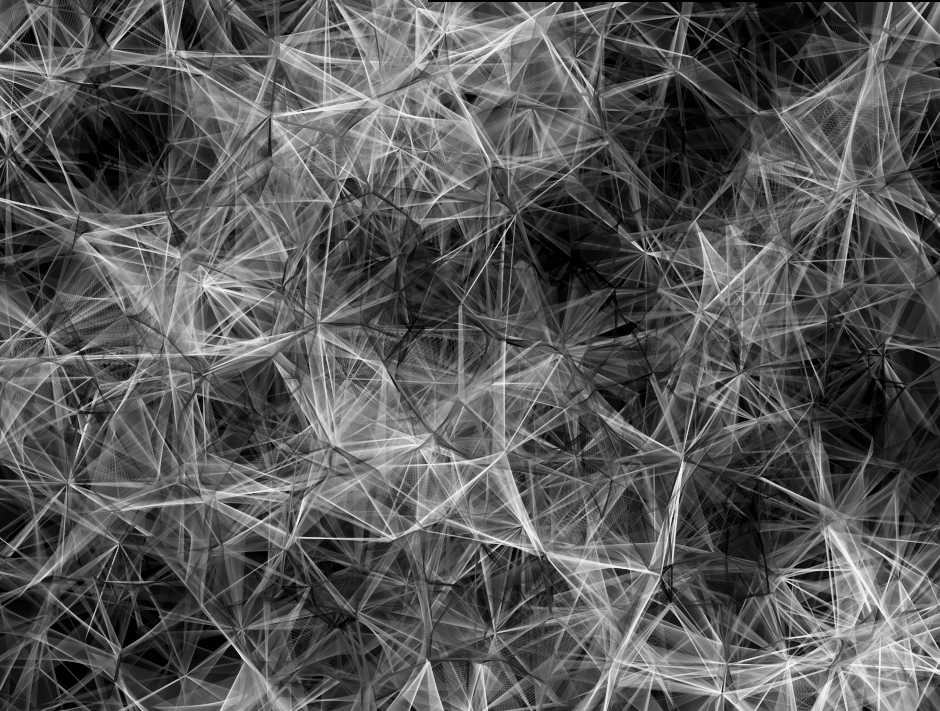
\includegraphics[width=1\paperwidth]{./images/portada.png}}
\begin{frame}[plain]
	\vspace{0.50\paperheight}
	\begin{titleBox}					
		\begin{beamercolorbox}[sep=2pt,center]{title}	
			\usebeamerfont{title}\textbf{Gracias por su atención!}\par
		\end{beamercolorbox}
	\end{titleBox}
\end{frame}

\end{document}
